%%%%%%%%%%%%%%%%%%%%%%%%%%%%%%%%%%%%%%%%%%%%%%%%%%%%%%%%%%%%%%%%%%%%%%%%%%%%%%%%
%%%%%%%%%%%%%%%%%%   Vorlage für eine Abschlussarbeit   %%%%%%%%%%%%%%%%%%%%%%%%
%%%%%%%%%%%%%%%%%%%%%%%%%%%%%%%%%%%%%%%%%%%%%%%%%%%%%%%%%%%%%%%%%%%%%%%%%%%%%%%%

% Erstellt von Maximilian Nöthe, <maximilian.noethe@tu-dortmund.de>
% ausgelegt für lualatex und Biblatex mit biber

% Kompilieren mit
% latexmk --lualatex --output-directory=build thesis.tex
% oder einfach mit:
% make

\documentclass[
  %tucolor,       % remove for less green,
  BCOR=12mm,     % 12mm binding corrections, adjust to fit your binding
  parskip=half,  % new paragraphs start with half line vertical space
  open=any,      % chapters start on both odd and even pages
  cleardoublepage=plain,  % no header/footer on blank pages
]{tudothesis}


% Warning, if another latex run is needed
\usepackage[aux]{rerunfilecheck}

% just list chapters and sections in the toc, not subsections or smaller
\setcounter{tocdepth}{1}

%------------------------------------------------------------------------------
%------------------------------ Fonts, Unicode, Language ----------------------
%------------------------------------------------------------------------------
\usepackage{fontspec}
\defaultfontfeatures{Ligatures=TeX}  % -- becomes en-dash etc.

% german language
\usepackage{polyglossia}
\setdefaultlanguage{english}

% for english abstract and english titles in the toc
\setotherlanguages{german}

% intelligent quotation marks, language and nesting sensitive
\usepackage[autostyle]{csquotes}

% microtypographical features, makes the text look nicer on the small scale
\usepackage{microtype}

%------------------------------------------------------------------------------
%------------------------ Math Packages and settings --------------------------
%------------------------------------------------------------------------------

\usepackage{amsmath}
\usepackage{amssymb}
\usepackage{mathtools}
\usepackage{textcomp}
% Enable Unicode-Math and follow the ISO-Standards for typesetting math
\usepackage[
  math-style=ISO,
  bold-style=ISO,
  sans-style=italic,
  nabla=upright,
  partial=upright,
]{unicode-math}
\setmathfont{Latin Modern Math}

% nice, small fracs for the text with \sfrac{}{}
\usepackage{xfrac}


%------------------------------------------------------------------------------
%---------------------------- Numbers and Units -------------------------------
%------------------------------------------------------------------------------

\usepackage[
  separate-uncertainty=true,
  per-mode=symbol-or-fraction,
]{siunitx}
\sisetup{math-micro=\text{µ},text-micro=µ}

%------------------------------------------------------------------------------
%-------------------------------- tables  -------------------------------------
%------------------------------------------------------------------------------

\usepackage{booktabs}       % \toprule, \midrule, \bottomrule, etc

%------------------------------------------------------------------------------
%-------------------------------- graphics -------------------------------------
%------------------------------------------------------------------------------

\usepackage{graphicx}
\usepackage{grffile}
% allow figures to be placed in the running text by default:
\usepackage{scrhack}
\usepackage{float}
\floatplacement{figure}{htbp}
\floatplacement{table}{htbp}

% keep figures and tables in the section
\usepackage[section, below]{placeins}


%------------------------------------------------------------------------------
%---------------------- customize list environments ---------------------------
%------------------------------------------------------------------------------

\usepackage{enumitem}

%------------------------------------------------------------------------------
%------------------------------ Bibliographie ---------------------------------
%------------------------------------------------------------------------------

\usepackage[
  backend=biber,   % use modern biber backend
  autolang=hyphen, % load hyphenation rules for if language of bibentry is not
                   % german, has to be loaded with \setotherlanguages
                   % in the references.bib use langid={en} for english sources
  sorting=none,
]{biblatex}
\addbibresource{references.bib}  % the bib file to use

\DefineBibliographyStrings{english}{andothers = {{et\,al\adddot}}}  % replace u.a. with et al.
\usepackage{bibstyle}
\usepackage{emptypage}
% Last packages, do not change order or insert new packages after these ones
\usepackage[pdfusetitle, unicode, linkbordercolor=tugreen]{hyperref}
\usepackage{bookmark}
\usepackage[shortcuts]{extdash}
%\usepackage{graphicx,subfigure}
%------------------------------------------------------------------------------
%-------------------------    Angaben zur Arbeit   ----------------------------
%------------------------------------------------------------------------------

\author{Christopher Krause}
\title{Track reconstruction for low energy protons using Corryvreckan}
\date{2021}
\birthplace{Mainz}
\chair{Lehrstuhl für Experimentelle Physik IV}
\division{Fakultät Physik}
%\thesisclass{Bachelor of Science}
%\submissiondate{12. Juli 2019}
%\firstcorrector{Dr.~Jens Weingarten}
%\secondcorrector{Prof.~Dr.~Dr.~Wolfgang Rhode}

% tu logo on top of the titlepage
\titlehead{\includegraphics[height=1.5cm]{logos/tu-logo.pdf}}

\begin{document}
\frontmatter
%\thispagestyle{empty}
\setcounter{page}{2}
\section*{Hinweise}
Empfohlen wird die Verwendung dieser Vorlage mit der jeweils aktuellsten TeXLive Version (Linux, Windows) bzw. MacTeX Version (MacOS).
Aktuell ist dies TeXLive 2016. Download hier:
\begin{center}
  \ttfamily\url{https://www.tug.org/texlive/}
\end{center}
Bei Verwendung von TexLive Versionen 2014 und älter sollte
die Zeile
\begin{center}
\verb+\RequirePackage{fixltx2e}+ 
\end{center}
als erste Zeile der Präambel noch vor der Dokumentenklasse eingefügt werden.
Dies lädt diverse Bugfixes für LaTeX, die ab TexLive 2015 Standard sind.

Die Vorlage \texttt{thesis.tex} ist für die Kompilierung mit \texttt{lualatex} ausgelegt, mit wenigen Anpassungen kann sie aber auch mit \texttt{pdflatex} oder \texttt{xelatex} verwendet werden. 
Die Dokumentenklasse \texttt{tudothesis.cls} kann mit allen drei Programmen verwednet werden.

Achten Sie auch auf die Kodierung der Quelldateien.
Bei Verwendung von Xe\LaTeX\ oder Lua\LaTeX\ (empfohlen) müssen die
Quelldateien UTF-8 kodiert sein.
Bei Verwendung von pdf\LaTeX\ nutzen Sie die Pakete \texttt{inputenc} und \texttt{fontenc} mit der korrekten Wahl der Kodierungen.

Eine aktuelle Version dieser Vorlage steht unter 
\begin{center}
  \ttfamily\url{https://github.com/maxnoe/tudothesis}
\end{center}
zur Verfügung.

Alle verwendeten Pakete werden im \LaTeX{} Kurs von Pep et al.\ erklärt:
\begin{center}
  \ttfamily\url{http://toolbox.pep-dortmund.org/notes}
\end{center}

Für Rückmeldungen und bei Problemen mit der Klasse oder Vorlage, bitte ein \emph{Issue} auf GitHub aufmachen oder eine Email an
\href{mailto:maximilian.noethe@tu-dortmund.de}{maximilian.noethe@tu-dortmund.de} schreiben.

Wenn Sie die Dokumentenklasse mit der Option \texttt{tucolor} laden, werden verschiedene Elemente in TU-Grün gesetzt.

\maketitle

% Gutachterseite
\makecorrectorpage

% hier beginnt der Vorspann, nummeriert in römischen Zahlen
\thispagestyle{plain}

\section*{Kurzfassung}
Die Protonentherapie ist, wegen ihrer höheren Präzision der Energiedeposition, eine wirkungsvolle Alternative zu herkömmlichen Röntgentherapie.
Auftretende Unsicherheiten durch die Verwendung von Röntgen Computertomographie können mit dem Verfahren der Protonen Computertomographie reduziert werden.
Um damit einen Bestrahlungsplan anfertigen zu können ist es nötig die Spuren der Protonen durch den Körper mithile von Detektoren zu rekonstruieren. \\
In dieser Arbeit wird die neue Spurrekonstruktions Software Corryvreckan mit der in Zukunft eingestellten Software EUTelescope auf ihre Funktionalität im
Rekonstruieren von Spuren in Testbeam Experimenten untersucht. Es wird gezeigt, dass Corryvreckan in der Lage ist Spuren mit vergleichbarer Qualität zu rekonstruieren.\\
Des Weiteren werden Simulation von Protonstrahlen durch ein Teleskop erstellt, um die rekonstruierbarkeit von niederenergetischen Protonen
mit Corryvreckan zu analysieren. (Hier noch Erbenis)

\section*{Abstract}
\begin{english}




\end{english}

\tableofcontents

\mainmatter
% Hier beginnt der Inhalt mit Seite 1 in arabischen Ziffern
\chapter{Introduction}
The investigation of particles and their properties is the foundation of particle physics. With the development of the standard model in the past century, particles
and their interactions with other particles could be better understood. The fundamental particles can be divided into quarks and leptons, making up the matter in the universe,
gauge bosons, which mediate three of the fundamental forces, and the Higgs boson.

In order to analyse interactions of particles, they are accelerated and brought to collision inside of particle colliders. The particles created in such collisions
can be detected with a surrounding detector system and thus the events can be reconstructed, giving an insight into their properties. It is, therefore, crucial to have
an optimal working detector to analyse the produced data precisely.
Currently, the largest collider is
the Large Hadron Collider (LHC) \cite{lhc} located at CERN, which is able to accelerate protons up to
a centre of mass energy of $\SI{14}{\tera\eV}$.
It operates since 2008 and helped particle physicists in finding the last missing particle of the standard model, the Higgs boson \cite{higgs}\cite{higgs_cms}, as well as giving more insight
into properties of particles like the top quark. Standard model parameters can be measured with greater precision, which improves the understanding of fundamental physical processes
and enables physicists to test their theories. %Physics beyond the standard model is also searched for at the LHC with great interest.

Besides the use of detectors in high-energy physics experiments, they are also a crucial part of medical equipment, specifically used for radiative treatments. \\
The idea to use protons as an effective particle for the treatment of cancer arose in 1946 \cite{1946} and over the years it proved to have several advantages over
conventional x-ray radiation therapy. To apply proton therapy, a radiation plan has to be created to determine the location of the tumor and the dose of the radiation.
For that purpose tomography scans create images of the inside of patients, enabling the precise irradiation of tumors.
The benefits of using protons for tomography scans in comparison to x-ray tomography scans for proton therapy caused a growing interest in this technique \cite{pbt}. \\
In order to create images with proton computed tomography, the reconstruction of proton tracks traversing the human body and the measurement of their energy is necessary.

This thesis focuses on the reconstruction of proton tracks under conditions present in proton computed tomography scans. To achieve that, the new track reconstruction software
Corryvreckan \cite{corryvreckan} is analysed based on its capability of reconstructing tracks in comparison to the EUTelescope framework \cite{gbl} known
for its long use in detector physics. Furthermore,
it is used to reconstruct
proton tracks, which are generated in Allpix$^2$ \cite{allpix} simulations to investigate the possibility of making proton computed tomography scans feasible with this framework.


%An interest for the imaging
%technique of proton computed tomogrophy came up around 1990, with proton therapy gaining in popularity due to its advantages over conventional x-ray therapy.
%In order to create images with proton computed tomography, the reconstruction of proton tracks traversing the human body is


%The ATLAS detector is one of the four large experiments at the LHC. % and the largest particle detector with a length of $\SI{46}{\meter}$ and a diameter of $\SI{25}{\meter}$.
%It was build to observe many different type of physical phenomena including the detection of the higgs boson in 2012 along with the CMS experiment. In order
%to identify the produced particles in the collisions, many layers of different detectors make up the entire ATLAS detector. The most inner layer is the pixel detector, which
%is composed of pixel sensor modules to detect particles and reconstruct their tracks.
%
%To measure the efficiency of pixel sensors,
%particle tracks are reconstructed in testbeam facilities with a telescope setup made of Mimosa26 pixel sensors to investigate the devices under test (DUT), which are
%placed inside the telescope. These measurements are necessary to ensure an optimal performance of sensor modules inside the experiments.

%\chapter{The Large Hadron Collider}
%%\section{Siliziumdetektoren}
%The LHC was build between 1998 and 2008 by the European Organization for Nuclear Research (CERN) in collaboration with 10000 scientist from over 100 countries
%and lies in a $\SI{27}{\kilo\meter}$ tunnel 175 metres underground in Switzerland near Geneva. It is a proton-proton synchrotron, which uses
%the systems to accelerate the protons before they are injected into the main accelerator. The linear particle accelerator LINAC 4 generates $\SI{160}{\mega\eV}$
%negative hydrogen ions and launches them into the Proton Synchrotron Booster (PSB). Here, the electrons are removed from the hydrogen ions, leaving only the nucleus
%consisting of one proton, which then enters the Super Proton Synchrotron (SPS). It increases the protons energy to $\SI{450}{\GeV}$ and feeds them to the
%LHC, where to opposing proton beams are accelerated. In the main ring,
%the protons are accumulated to bunches and accelerated to their maximum energy of $\SI{13}{\tera\eV}$ in 20 minutes.
%
%At four locations, the two proton beams
%are crossed, making it possible for them to collide. Around these interaction points, the four large experiments, ATLAS, CMS, LHCb and Alice are operated.
%Occasionaly lead nuclei are accelerated to study matter under extreme conditions at the ALICE experiment. The ATLAS and CMS experiment are general-purpose detectors for
%high energy physics. They differ on their technical design to achieve their goal and enable to corrobate each others results.
%LHCb is an asymmetric particle detector specialized in measuring the parameters of CP violation in B-meson decays.
%Further experiments at the LHC include TOTem, LHCf, MoEDAL and FASER, which focus on specialized research. Figure \ref{fig:lhc_aufbau} shows a schematic depiction
%of the LHC.
%
%\begin{figure}[H]
%  \centering
%  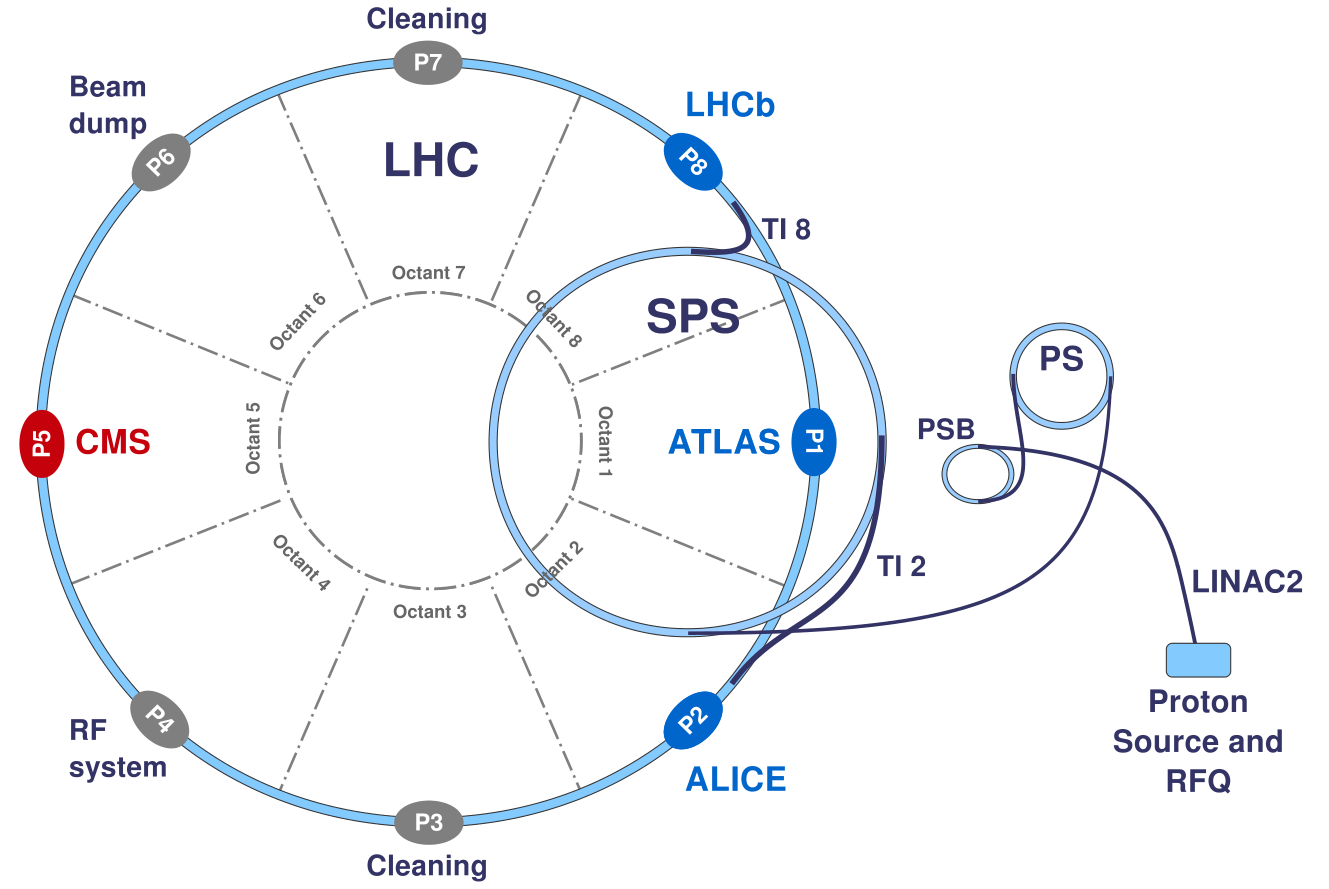
\includegraphics[height=0.4\textwidth]{images/lhc_aufbau.png}
%  \caption{Schematic representation of the CERN accelerator complex (not to scale)\cite{lhc_aufbau}.}
%  \label{fig:lhc_aufbau}
%\end{figure}
%
%After the second run from 2015 to 2018 followed the Long Shutdown 2 (LS2) until 2021 in order to upgrade the accelerator. The goal is to increase the luminosity by a factor of 10 by
%implementing High Luminosity Large Hadron Collider (HL-LHC) in the Long Shutdown 3 (LS3), which is planned to be operational in 2026. Figure \ref{fig:lhc_plan} shows the timeline
%of LHC programme.
%
%\begin{figure}
%  \centering
%  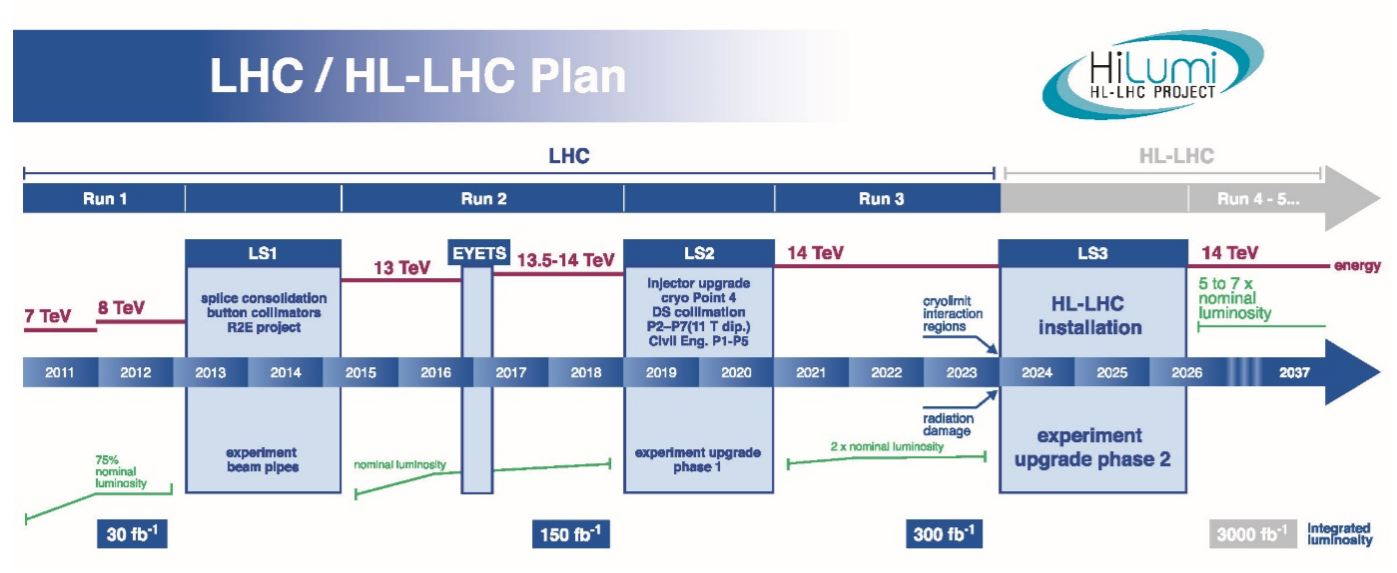
\includegraphics[height=0.4\textwidth]{images/lhc_plan.png}
%  \caption{Timeline of the operational phases and Shutdowns of the LHC. The energy of accelerated protons in each phase is shown in red and the luminosity in green \cite{lhc_plan}.}
%  \label{fig:lhc_plan}
%\end{figure}
%
%\section{The ATLAS detector}
%The ATLAS detector is the largest general-purpose detector with a length of $\SI{46}{\meter}$ and a diameter of $\SI{25}{\meter}$.
%It was designed to be a cylindric $4\pi$ detector, covering up most of the solid angle to detect particles flying in all directions.
%Both ATLAS and CMS detected the Higgs Boson in 2012 and thus prove the existence of the last missing particle of the standard model.
%Further goals of the detector is to search for beyond the standard model physics in the high energy domain, where current theories possibly break down.
%Top quarks, which were produced at the LHC in large amount of quantities for the first time, can be studied more precisely with the help of the ATLAS detector.
%
%The entire detector is made out of four different layers of detector systems, the Inner Detector, the electromagnetic and hadronic calorimeters
%and the muon spectrometer. Only a couple of centimeter away from the interaction point lies the Inner Detector with its purpose to track the produced charged particles.
%It is made of three subsequent components, with the innermost layer called the Pixel Detector and consists of three layers of silicon pixel detectors. The middle constituent
%is the Semiconductor Tracker (SRT) with a similar purpose. Here, four layers of silicon stripe detectors are used for detection, while they have a lower spatial resolution, a larger
%area can be covered with them more efficiently. The Transition Radiation Tracker (TRT) is the outermost component and uses straw detectors for tracking as well as materials with
%different refractive index inbetween the straws. Relativistic particles will produce transition radiation by traversing these materials, which enables particle
%identification, especially for light charged particles.
%A magnetic solenoid surrounding the Inner Detector produces a $\SI{2}{\tesla}$ magnetic field to curve the trajectories of charged particles in order to determine their
%momentum. \\
%The electromagnetic calorimeter is positioned outside the magnetic field and aims at absorbing electrons, positrons and photon induced
%electromagnetic showers in order to measure the energy of the initial particle. Lead and stainless steel serve as the energy absorbing material and liquid argon as the
%sampling material. Hadrons tend to traverse the electromagnetic calorimeter without losing all their energy, which is the reason the hadronic calorimeter comes after.
%It uses steel as sampling material and scintillating tiles to measure the energy. \\
%Because muons easily pass both calorimeters, the outermost detector system is the muon spectrometer consisting of silicon detectors to track the muons and three toroidal magnets
%building up a magnetic field for momentum measurement. Figure \ref{fig:atlas} ilustrates the ATLAS detector with its components.
%
%\begin{figure}
%  \centering
%  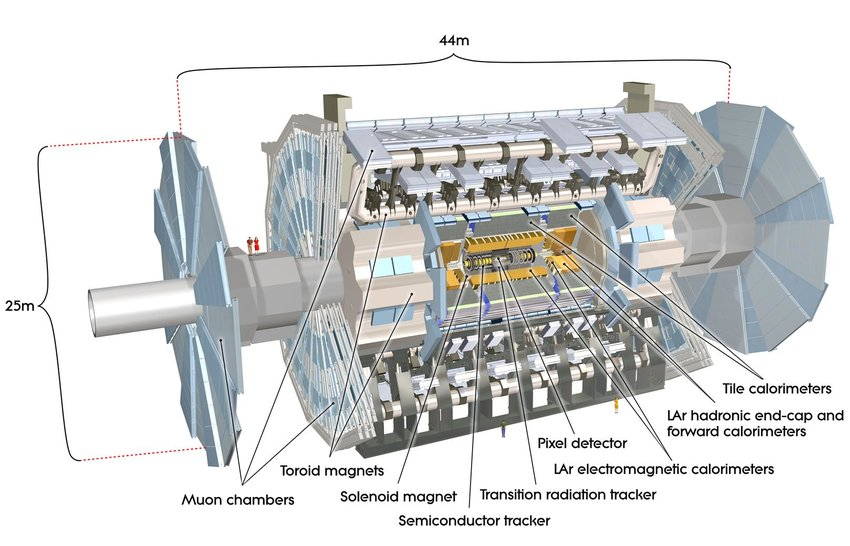
\includegraphics[height=0.5\textwidth]{images/atlas.png}
%  \caption{Illustration of the ATLAS detector and its subsequent components. Two Humans are depicted at the bottom for a size comparison \cite{atlas}.}
%  \label{fig:atlas}
%\end{figure}
%
%During the Long Shutdown 3 of the LHC, the ATLAS Inner Tracker (ITk) upgrade is planned to be installed. Its goal is to perform as good or better as the current detector, while
%withstanding the harsher environment of the HL-LHC.

\chapter{Radiation therapy}
Radiation therapies are medical treatments using ionizing radiation mainly to kill cancer cells in patients. The ionising particles interact with the
cancer cells to damage their DNA causing cellular death. These treatments focus on cancer that is localized to one area inside the body. \\
The type of particle used in radiation therapy is crucial to the overall treatment due to the different interactions of particles with the human body.
Photons, specifically x-rays, are the most common particles being used for radiation therapy.
A newer alternative is proton therapy, due to the different properties of protons giving advantages over conventional x-ray therapy explained in the following section.

\section{Proton therapy}
Proton therapy is external beam radiotherapy using a proton beam for irradiation. While proton therapy centres have only been used since 1889 the technological
advancement ensures the continual rise of hospitals offering proton therapy.
The proton therapy centres either use cyclotrons or synchrotrons to accelerate the protons, with the former being compact and simple to operate and the latter being able
to produce protons of varying energies from $\SI{50}{\MeV}$ to $\SI{250}{\MeV}$.
Unlike photons, which tend to deposit their entire energy in a single ionisation process, protons undergo multiple Coulomb scattering inside matter. The
energy loss of protons is inversely proportional to the square of their velocity, which causes them to deposit most of their energy on the last millimeters of their path.
This behaviour is called the Bragg peak and is shown in figure \ref{fig:bragg}. Regulating the energy of the protons allows for precise control of the Bragg peak depth inside
the human body. Thus, using multiple proton energies in the proton beam enables a uniform energy deposition inside the target volume.

\begin{figure}
  \centering
  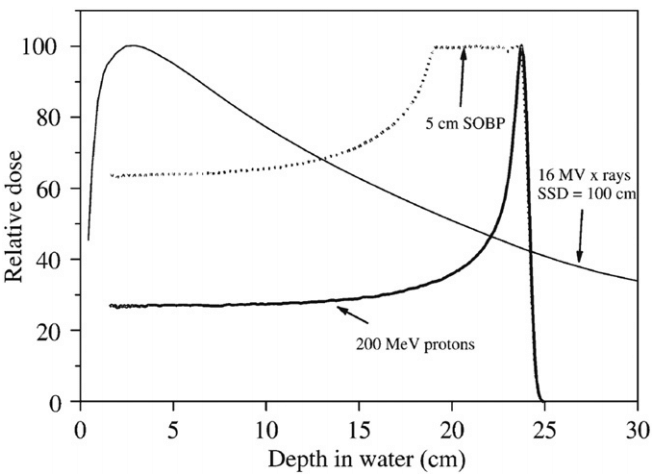
\includegraphics[height=0.6\textwidth]{images/tiefendosis.png}
  \caption{A Radiation dose of unmodulated $\SI{200}{\mega\eV}$ protons and with a $\SI{5}{\centi\meter}$ spread-out Bragg peak (SOBP)
  as a function of the penetration depth in water. In comparison, the energy deposition of a $\SI{16}{\mega\volt}$ x-ray beam \cite{bragg}.}
  \label{fig:bragg}
\end{figure}
Due to this property, protons enable irradiating tumors with greater precision than with
x-rays, as surrounding healthy tissue is less damaged, especially behind the tumor. Figure \ref{fig:risk} shows the irradiated areas of a brain for conventional and
proton therapy to emphasise their differences.

\begin{figure}
  \centering
  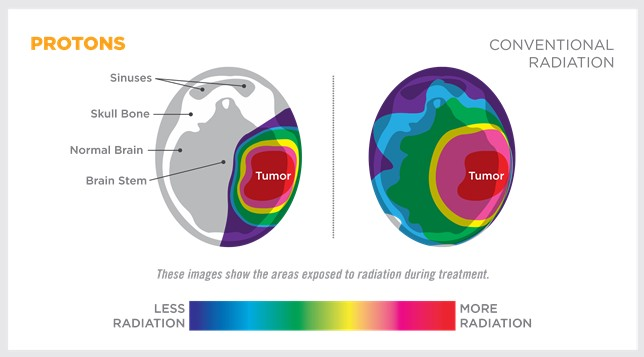
\includegraphics[height=0.5\textwidth]{images/risk.png}
  \caption{Radiated region for protons and x-rays to treat a brain tumor. The irradiation for proton therapy is far more precise and damages less healthy tissue than
  x-ray therapy.}
  \label{fig:risk}
\end{figure}


\section{Computed tomography} \label{sec:ct}
To irradiate a patient save and efficiently it is necessary to create an irradiation plan by identifying the tumor and the surrounding healthy tissue. In order to do so, a computed
tomography (ct) scan is performed using a particle beam to create an image of the region encompassing the tumor. For x-ray therapy as well as proton therapy x-ray ct scans
are used primarily. \\
To create an image, the patient lies within a rotating x-ray tube, the gantry, which generates x-ray beams to irradiate the specific volume. The gantry also
includes a row of detectors measuring the photons after traversing the human body. Due to the fact that different tissue materials inside the body absorb a different
amount of light, a projection of the irradiated volume can be created. By rotating the x-ray tube, projections are created from many different angles around the patient.
Unlike in radiography, where two-dimensional projections are produced, ct scan measurements are one-dimensional absorption profiles. The sum of the profiles contains
the entire information of the inside structure, but can not be interpreted directly. Projections and the original three-dimensional structure are connected through
the inverse radon transformation. An implementation of that algorithm is the filtered back projection:
\begin{align}
  f(x,y) = \int_0^{\pi} \left(\int_{-\infty}^{\infty} p_{\phi}(z') \cdot g(z - z') \mathrm{d}z'\right) \mathrm{d}\phi
\end{align}
Where $f(x,y)$ is the original image, $p_{\phi}(z)$ the projection in the direction of the angle $\phi$ and $g(z)$ a high-pass filter. However, the inverse
radon transformation is an ill-posed problem, which demands an irregular filter kernel g(z). To solve this problem in praxis, a fast convolution algorithm is used for the
filtered back projection. This means that the projection is multiplied with the high-pass filter in Fourier space, where each frequency component is weighted proportional to their
absolute value. In the end, each one-dimensional projection is stretched into two dimensions and rotated around the angle $-\phi$. The sum over all projections will yield the
final image.


\section{Proton computed tomography}
Creating irradiation plans for proton therapy with x-ray ct images causes larger uncertainty due to the different stopping powers of the particles.
To compensate for the differences, a range uncertainty margin is applied to the prescribed range, which increases with greater travel distance through the body. This
method is shown in figure \ref{fig:paganetti}.

\begin{figure}
  \centering
  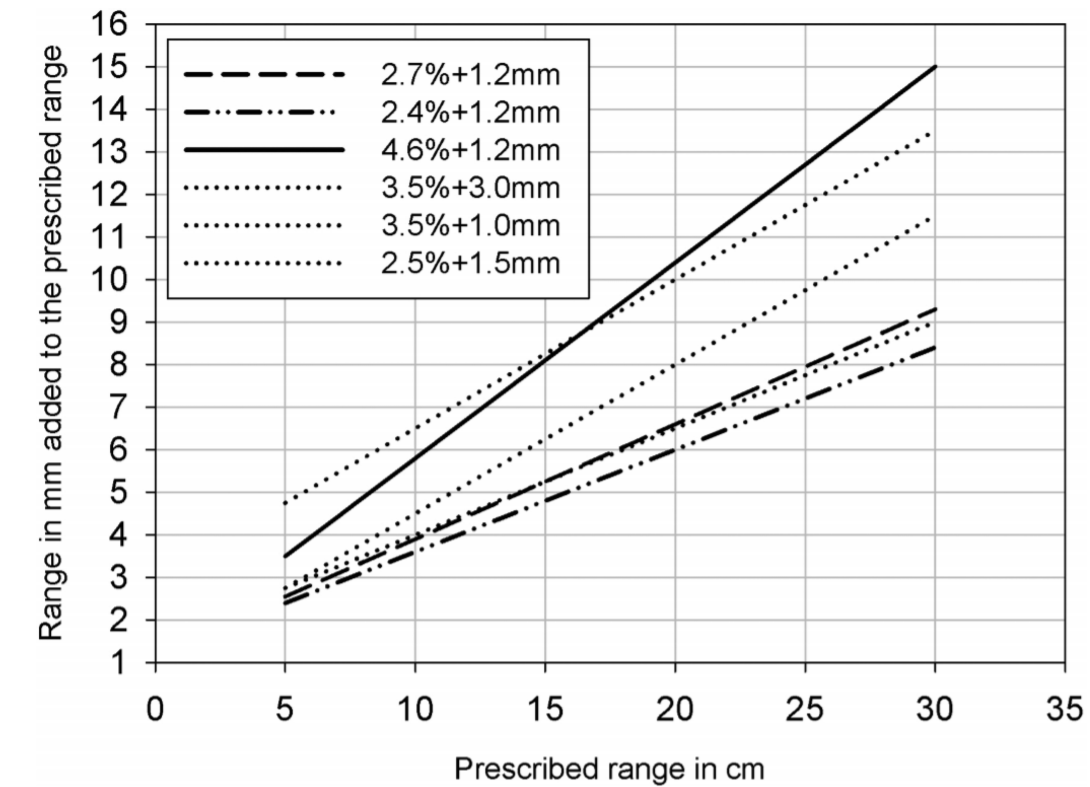
\includegraphics[height=0.6\textwidth]{images/prescription.png}
  \caption{Applied uncertainty margins at the Massachusetts General Hospital (3.5\,\% +
1mm), the MD Anderson Proton Therapy Center in Houston (3.5\,\% + 3mm), the Loma Linda
University Medical Center (3.5\,\% + 3mm), the Roberts Proton Therapy Center at the
University of Pennsylvania (3.5\,\% + 3mm), and the University of Florida Proton Therapy
Institute (2.5\,\% + 1.5mm), shown as dashed lines. Dashed-dotted and dashed line: Uncertainty margin for with and without the use of Monte Carlo dose calculation.
The solid-line describes the safety margin for complex geometries without Monte Carlo dose calculation \cite{paganetti}.}
  \label{fig:paganetti}
\end{figure}

Since the position of the protons energy deposition has to be determined as precisely as possible to minimise damage dealt to healthy tissue, a computed tomography scan using protons
is a promising alternative to conventional ct. Creating an image with proton ct is similar to conventional. A proton beam irradiates and deposits energy in the patient. The
protons remaining energy is then measured with a calorimeter system behind the patient to gain information about the composition of the tissue. A projection can be created,
if the proton's tracks can be reconstructed. However, due to multiple Coulomb scatterings of the protons inside the patient, the spatial resolution will decrease in comparison
to conventional ct. Numerous projections are created by varying the angle of the proton beam with respect to the target. The entire setup is schematically in figure \ref{fig:proton_ct}.

\begin{figure}
  \centering
  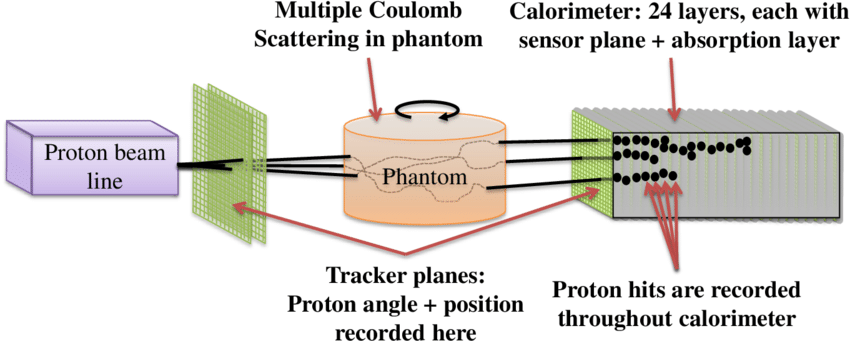
\includegraphics[height=0.4\textwidth]{images/proton_ct.png}
  \caption{Procedure of the proton computed tomography. The tracker planes are used to reconstruct the proton tracks and the calorimeter to measure their remaining energy.
  The phantom is the placeholder of a patient \cite{proton_ct}.}
  \label{fig:proton_ct}
\end{figure}

The different projections can then be reconstructed to a complete image of the irradiated volume as explained in section \ref{sec:ct}.
This thesis focuses on the track reconstructions of the low energy protons used in proton computed tomography and whether they can be reconstructed accurately.
In the following chapter, the track reconstruction of particles is adressed in more detail.

\chapter{Testbeam}
Studying the properties of sensor modules is crucial for an optimal performance of particle detectors. The new pixel modules used for the ATLAS ITk upgrade have to be thoroughly
tested in terms of efficiency and radiation hardness in order to fulfill the necessary requirements for their installment.
In order to evaluate the sensors performance they are irradiated in testbeam experiments similar to the conditions in the LHC.
These beam test measurements are performed mainly in two testbeam facilities, being located at Cern and Deutsches Elektronen Synchrotron (DESY). Sensors that are planned to be
installed in the ATLAS ITk are tested at DESY during the LS2.

\section{DESY Testbeam}
DESY is a national research center located at Hamburg. It operates the electron synchrotron DESY II since 1987 initially to accelerate electrons before injecting them into
HERA, the largest synchrotron at DESY. After the shut down of HERA in 2007, DESY II is now used for testbeam measurements. It produces an electron beam with energies upto
$\SI{7}{\GeV}$, which collides with a carbon fiber target creating bremsstrahlung in the process. The photons are extracted and collide with a secondary target
converting them to electron positron pairs. A dipole magnet behind the target creates a homogenous magnetic field to filter out unwanted energies and particles. This process
is shown schematically in figure \ref{fig:testbeam}.

\begin{figure}
  \centering
  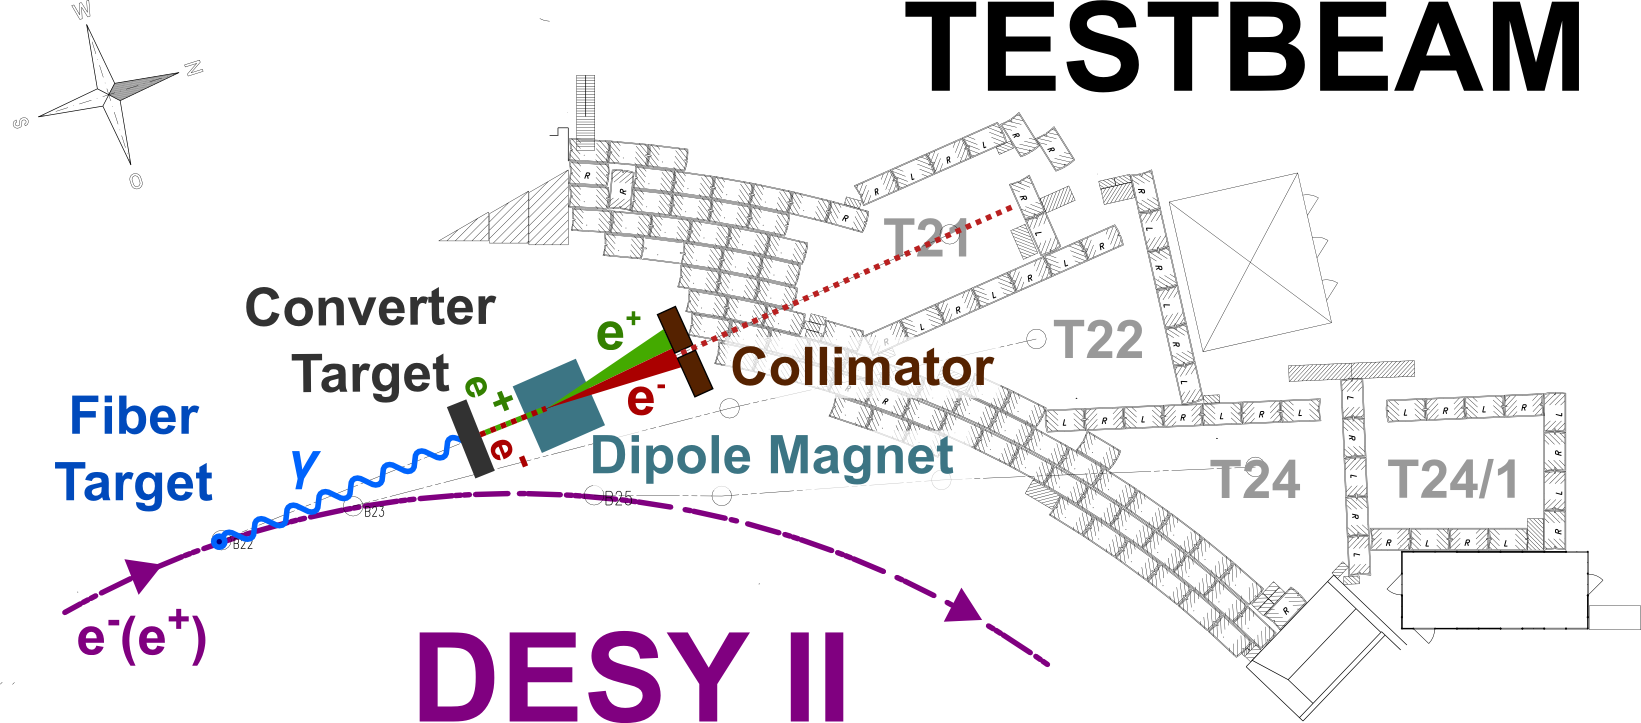
\includegraphics[height=0.4\textwidth]{images/desy.png}
  \caption{Depiction of the beam generation in testbeam experiments going through the beam line TB21 \cite{testbeam}.}
  \label{fig:testbeam}
\end{figure}

The permantly installed EUDET-type Pixel Beam telescopes DATURA and DURANTA are located behind the beam lines TB21 and TB22 and enable the tracking of the particles
produced by DESY II. Both telescopes consist of six Mimosa26 monolithic active pixel sensors with %a pixel pitch of $\SI{18.4}{\micro\meter} \times \SI{18.4}{\micro\meter}$.
three sensors each incorporated into one arm of the telescope and the DUT's being placed inbetween. A polystyrene box filled with dry ice is used to cool the DUT's to
avoid annealing and other unwanted effects due to heat. For time references during the measurements, an FE-I4 sensor is placed behind the telescope with a
time resolution of $\SI{25}{\nano\second}$ The sensors contain $336 \times 80$ pixels with a
$\SI{50}{\micro\meter} \times \SI{250}{\micro\meter}$ pixel pitch. Figure \ref{fig:telescope} shows the telescope setup of DATURA.

%\begin{figure}
%  \centering
%  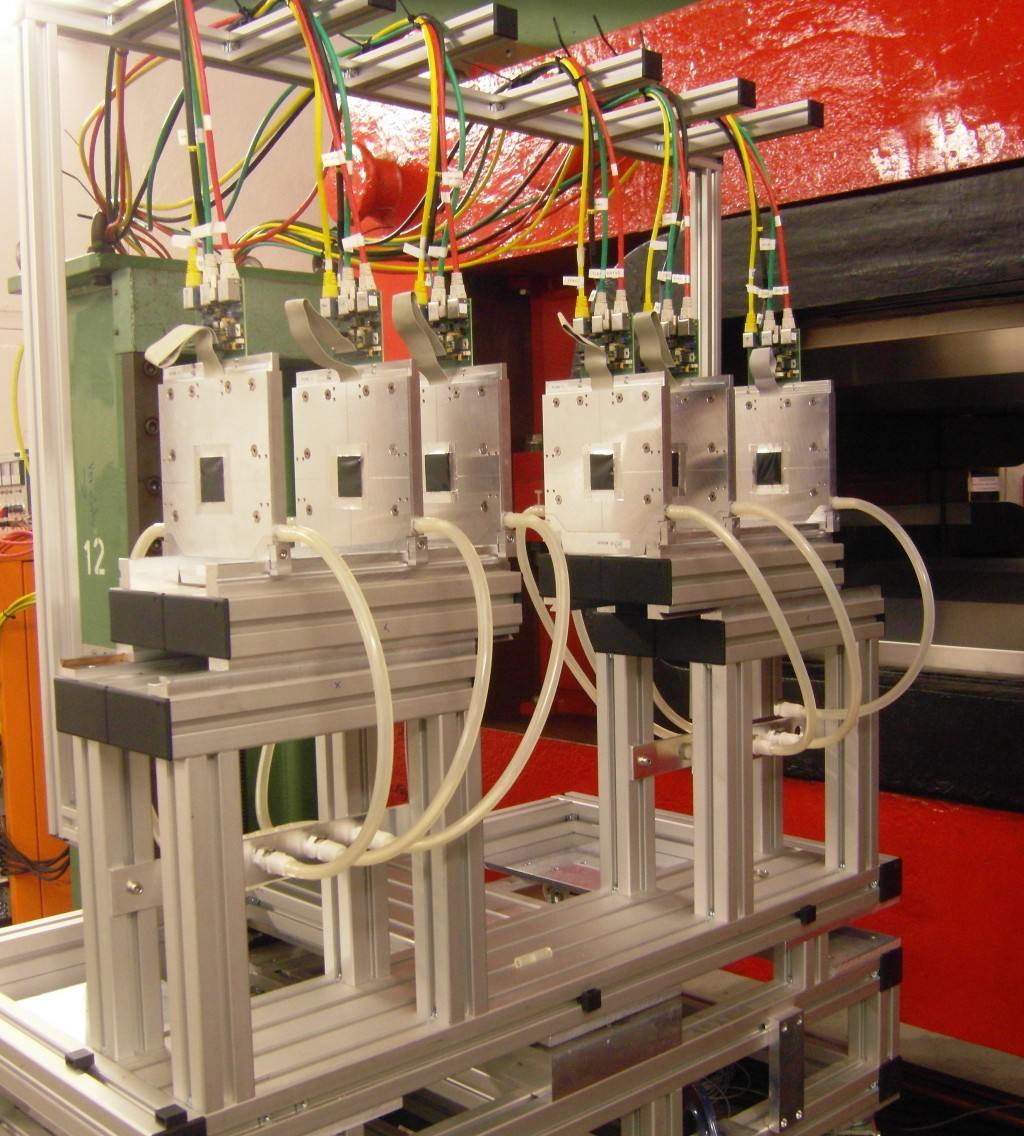
\includegraphics[height=0.4\textwidth]{images/telescope.jpg}
%  \caption{Shown is the Beam telescope DATURA consisting of six Mimosa26 sensors placed in the jigs. The tubes connected to the sensors transport water to
%  cool the sensors \cite{telescope}.}
%  \label{fig:telescope}
%\end{figure}

\begin{figure}
  %\centering
  \begin{subfigure}{0.48\textwidth}
      \centering
      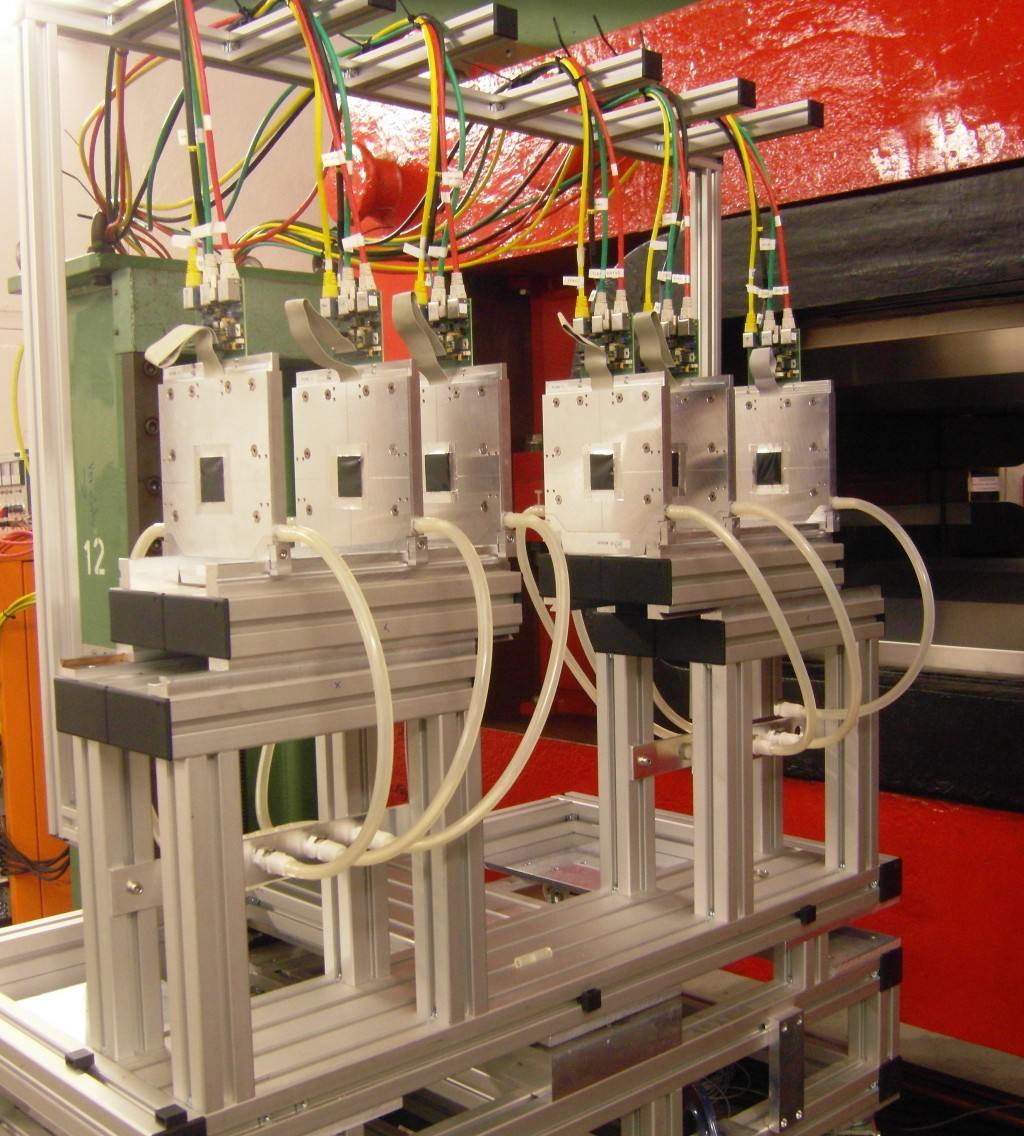
\includegraphics[height=0.82\textwidth]{images/telescope.jpg}
  \end{subfigure}
  \begin{subfigure}{0.48\textwidth}
      %\centering
      \hspace{-1cm}
      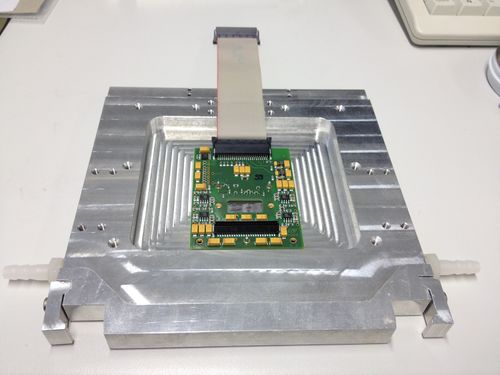
\includegraphics[height=0.82\textwidth]{images/mimosa.jpg}
  \end{subfigure}
  \caption{Shown on the left is the Beam telescope DATURA consisting of six Mimosa26 sensors placed in the jigs. The tubes connected to the sensors transport water to
  cool the sensors \cite{telescope}. Shown on the right is the Mimosa26 board inside the aluminium housing \cite{mimosa}. }
  \label{fig:telescope}
\end{figure}

Mimosa26 are fabricated in a standard $\SI{0.35}{\micro\meter}$ CMOS process with a fast binary read out
%size of $\SI{13.7}{\milli\meter} \times \SI{21.5}{\milli\meter}$.
Signals are measured with a time resolution of $\SI{230}{\micro\second}$ with each measurement in a read out cycle belonging to the same event.
They contain $576 \times 1152$ pixels with a pixel pitch of $\SI{18.4}{\micro\meter} \times \SI{18.4}{\micro\meter}$
and a thickness of $\SI{50}{\micro\meter}$.

The generic data aquisition framework EUDAQ records the data produced in testbeam experiments. Its centrally handles the data flow and synchronises data stream to enable
the integration of different independent devices under test. An exemplary setup of a beam telescope with EUDAQ is shown in figure \ref{fig:eudaq_bild}.
More information in \cite{eudaq}.

\begin{figure}
  \centering
  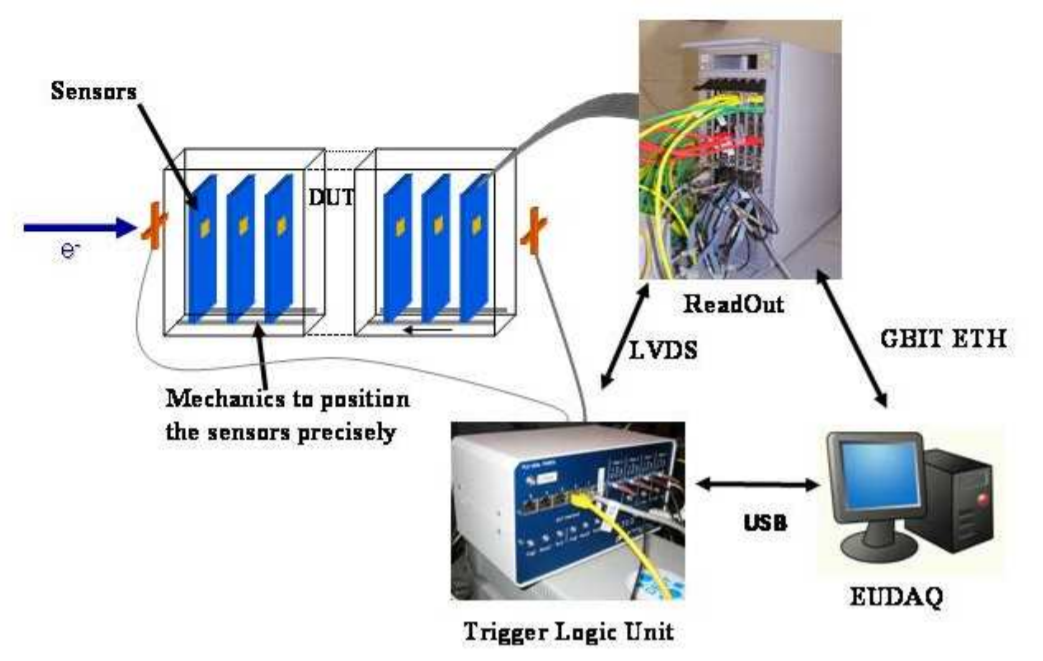
\includegraphics[height=0.4\textwidth]{images/eudaq.png}
  \caption{Necessary components for an analogue telescope \cite{eudaq_bild}.}
  \label{fig:eudaq_bild}
\end{figure}

\chapter{Track reconstruction}
The hit information of the sensor planes can be used to reconstruct the initial particles track. To properly reconstruct the tracks, multiple steps have to
be performed. For that reason entire frameworks were created to allow for a versatile and accurate track reconstruction to be possible. Two of the most
developed reconstruction softwares were used in this thesis and are explained in the following.

\section{The track reconstruction framework EUTelescope}
In order to do that the sotware EUTelescope was developed and
primarily used since 2007. It uses the Modular Analysis and Reconstruction for the Linear Collider (MARLIN) framework, which is part of the
International Collider Software package (ILCSoft). Each step in the reconstruction depends on MARLIN processors, which read in data, modifies and outputs new data to be
taken by the next processors. The individual steps in the reconstruction will call on certain processors specified for its task resulting in a
modular structure.

Information about the telescope geometry is stored in  Geometry API for Reconstruction (GEAR) files. This includes the position and rotation
of the sensors as well as their pixel layouts. Further parameters like radiation hardness, magnetic field and general properties of the used sensors have to be
specified to ensure proper track reconstruction.

General parameters and parameters in individual reconstruction steps are specified in the configuration file. This includes the import of the raw data and the
geometry file, the applied reconstruction steps and the definition of the cuts. \\
The steering files define the processors used in each reconstruction step and in which order they are executed.
A complete track reconstruction with EUTelescope contains the converter, the clustering, the hitmaker, the alignment and the track fitting in this respective order.
The overall track reconstruction of EUTelescope is shown in figure \ref{fig:track_reco} with the most important steps explained in the following.

\begin{figure}
  \centering
  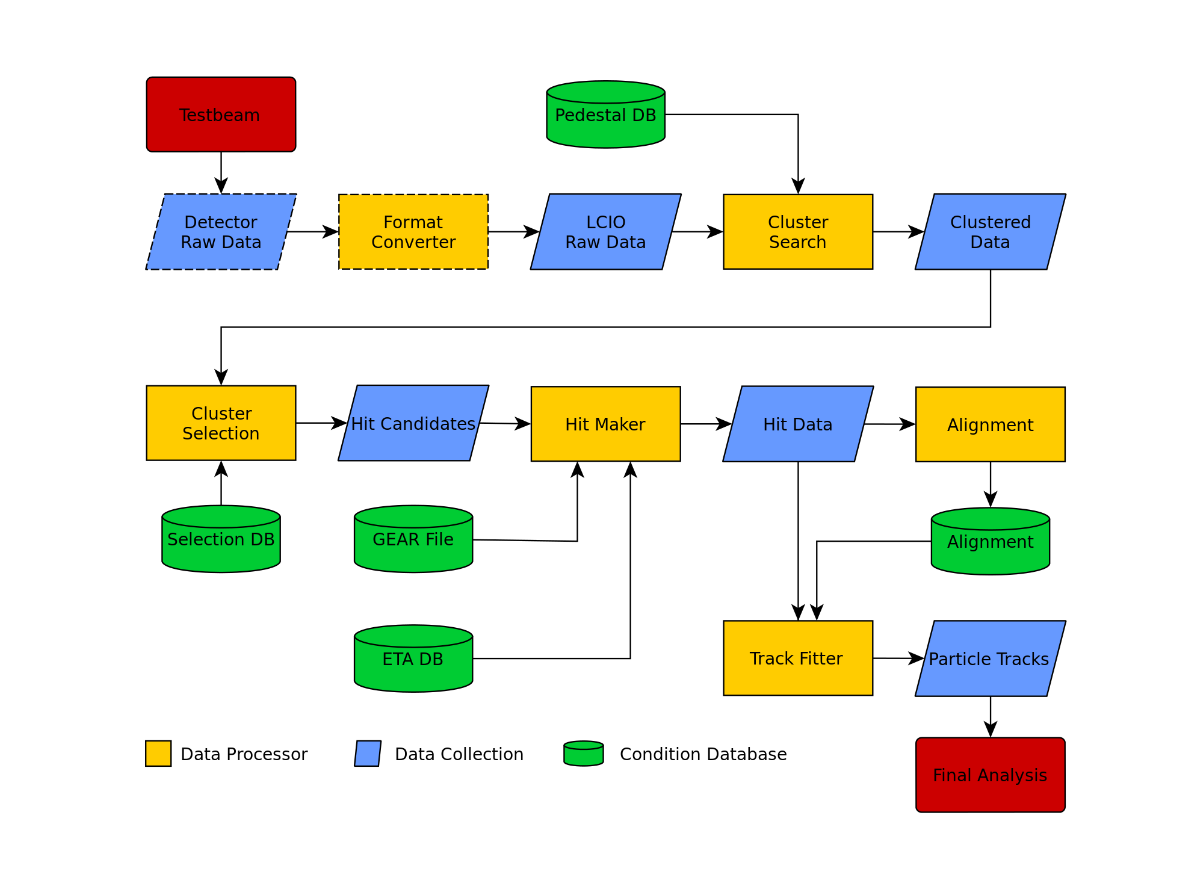
\includegraphics[height=0.6\textwidth]{images/track_reco.png}
  \caption{The overall track reconstruction of EUTelescope including the MARLIN processors and files. \cite{track_reco}.}
  \label{fig:track_reco}
\end{figure}

First, the raw data has to be converted to the lcio format for subsequent MARLIN processors. In addition, the module detects noisy pixels by analysing the
hit rate of the pixels and dividing them by the sum of measured events. The resulting firing frequency can be limited by user defined cuts, thus removing entries
from noise considered pixels from the lcio file.

In the clustering process, hit information on a sensor plane generated by the same particle will be clustered. Cluster with more than one pixel occur due
particles traversing through multiple pixels or charge sharing. Pixels will be grouped together based on their distance.
Regulation of the clustering process is then possible with cuts on the pixel distances.

The hitmaker step determines the particles hit position, the cluster center, of each cluster. For one pixel cluster, the cluster center is equal to the middle of
te pixel. Cluster centers of clusters with more than one pixel are calculated with a charge weighted center of gravity algorithm. This means, that
the deposited charge of each pixel is taken into account to derive the particles position. The cluster centers are transformed to the global coordinate
system of the telescope to function as the hit position for the track reconstruction. Global hit information on the sensors of particle tracks is assumed to be correlated with only
a small spread of the beam angle, which makes an initial guess of the telescope alignment, the prealignment, possible. With the prealignment it is possible
to correct larger misplacements of the sensors.

To compensate possible misaligment of sensors in the telescope, the alignment processor tries to optimise the setup. Cluster information from the hitmaker
are used to fit tracks through the planes and correct deviations by rotating and shifting the sensors. After the alignment process is finished a new gear file is produced, which
is then used for further reconstruction steps. Usually, several iterations of the alignment process occur to determine the optimal positions of the sensor planes
in the telescope.
There are two major processors for the alignment step, which implement different track fitting algorithms.
The DAF processor is based on a Kalman filter and was specifically designed for high noise environments. It uses the inbuild combinatorics filter, which fits
straight line tracks through all combinations of clusters allowed by the specified cuts and only keeps the ones with a minimum $\chi^2$. Here, the $\chi^2$ parameter
describes the goodness of the fit and is defined as:
\begin{align}
  \chi^2 = \sum_i (r_x/\sigma_x)^2 + (r_y/\sigma_y)^2
\end{align}

The parameters $r_x$ and $r_y$ refer to the residuals on each sensor in X and Y direction, which describe the distance of the cluster center used for the track fit and the
position of the track on a plane. All residuals are weighted with their spatial resolution $\sigma_x$ and $\sigma_y$ for each sensor. \\
The second fitter uses the General Broken Line (GBL) algorithm with a separate patter recognition processor for track fitting. Kinematics of
beam particles are used to predict hits belonging to a track. In the track finding process, two straight lines are fitted through the upstream and
downstream sensors, whenever the user defined cuts on the slope allow it. The two straight lines are extrapolated to the centre of the telescope, where
they form the overall track depending on their distance to each other and the corresponding user defined cut.\\
Fitted tracks used for the alignment are handled by the Millipede II processor. It performs least squares minimisation for a particular set of problems, which
have an interest of global parameters over local parameters in common. Thus, Millepede II is able to align the planes with any applied track model.

After the alignment is finished the tracks are fully reconstructed with either the DAF or the GBL fitter. Optionally, DUT's can be included in the fitting
process, however it is usually avoided to keep the residuals of the DUT unbiased. In the scope of this thesis, the GBL processor is used for the
alignment and fitting step. To reconstruct a track, the fitGBL processor uses GBL points, which carry a series of attributes. These points can either be a
hit or an other point of interest on the trajectory. Figure \ref{fig:gbl} depicts an exemplary reconstructed track with the fitGBL processor.

\begin{figure}
  \centering
  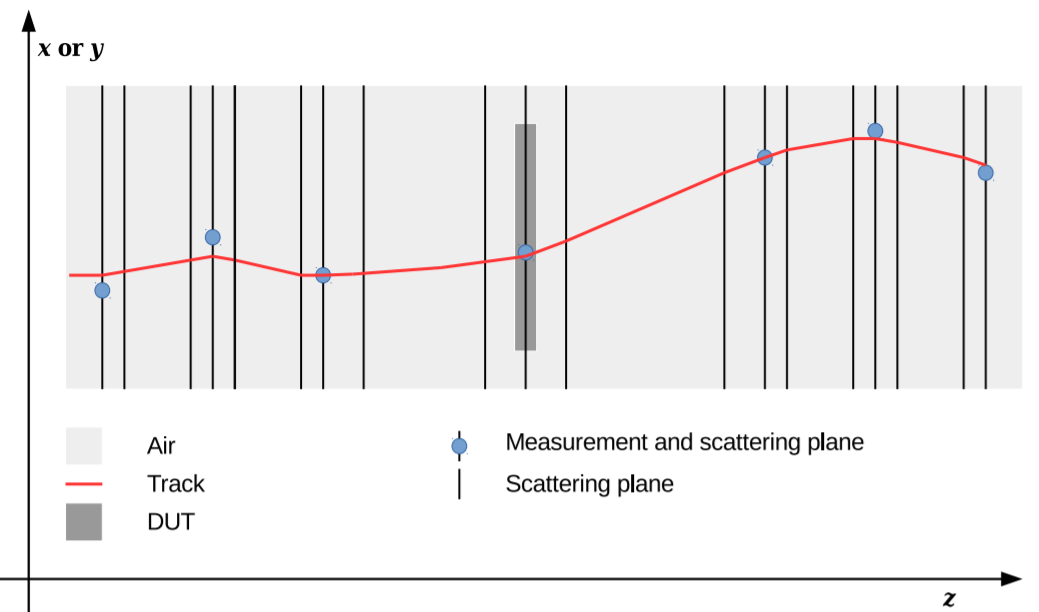
\includegraphics[height=0.5\textwidth]{images/gbl.png}
  \caption{Track reconstruction with the fitGBL processor. Scatterering points are connected with a straight line. \cite{gbl}.}
  \label{fig:gbl}
\end{figure}



\section{The track reconstruction framework Corryvreckan}
Corryvreckan is a fast and lightweight track reconstruction framework released in 2017 and is the most developed alternative to the EUTelescope software.
Since the development and support of the EUTelescope discontinued, Corryvreckan is planned to supersede the former as the primarily used track
reconstruction software. Its main advantage is the minimal amount of external dependencies connected to the software and the more user friendly usage of
it.
Corryvreckans structure is based on the modular concept of the simulation software Allpix$^2$, making the software flexible and ensures to meet the requirements for track reconstruction in
complex environments. Global parameters and modules used for the track reconstruction are specified in the configuration file, which starts the event loop upon
executing. Data and the geometry of the setup are both imported into the configuration file as well. A reference sensor has to be specified in the geometry folder
for which the rest of the telescope is aligned with.

During event processing, information taken and produced by the modules are temporarily stored on the clipboard, serving as the infratructure for temporary
storing information. %the event, the
%temporary data storage and the persistent storage. The event is the central element storing information about the currently processed data.
The necessary steps in the track reconstruction chain of the software are similar to ones taken in EUTelescope and are explained in the following.

To load the taken data into Corryvreckan a certain eventloader module is used depending on the data format. The order of Eventloader modules
is important as the first module loaded will define the event on the clipboard either through trigger numbers or a time window. Measurements stored with EUDAQ are loaded with the
EventloaderEUDAQ module, which requires the EUDAQ library as an external dependency. Altneratively to the eventloader modules, data in root format can also be imported
with the FileReader module, which is mainly used for simulated data or data written out with the FileWriter module.

The clustering process can be either done with the Clustering4D or the ClusteringSpatial module, with the former being the standard clustering module taking hit timestamps
into account. Spatial and timing cuts can be defined by the user either through absolute values or relative factors multiplied by the sensors spatial and time resolution. Both
center of gravity or arithmetic mean calculations for the cluster centre can be chosen.


While not mandatory for the overall track reconstruction chain, a correlation module can be applied to create several correlation plots, taking the hit information
from the clipboard to plot their location against the ones of the reference sensor. These plots can then be used to identify major translational and
rotational misalignments of sensors.  Either an abolute or relative time cut can be specified for clusters on a sensor to be considered in respect to
the reference sensor.

The Prealignment module accounts for major tranlational misplacements of sensors and performs translational shifts along the X and Y axis of up to several millimeter to ensure a proper alignment later on, as higher misaligmnents might cause the main alignment process to not converge correctly.
To calculate the applied shifts, the mean of the 1D correlation
histograms of each detector is used. A  relative or absolute time cut can be specified.

Reconstructing tracks from cluster centres can then be accomplished with the Tracking4D or Trackingspatial module. Similar to the clustering modules, only the former
takes timestamp information into account and is therfore the standard track reconstruction module. For the track finding process, clusters on the first plane are
related to clusters close in time on subsequent planes using straight lines.
The Tracking4D module has two possible track models, straight lines as default setting and general
broken lines, for fitting. General broken lines account for multiple coulomb scattering and considers scattering at every sensor plane as well as the surrounding air.
Absolute and relative spatial and time cuts can be specified, as well as the minimum number
of clusters necessary to fit a track. The DUT can be included reconstruction process, though this is avoided in this thesis to keep the residuals of DUT's unbiased.


To align the telescope, the AlignmentTrackChi2 module is used. It performs rotational and translational telescope
alignment according to minimise the $\chi^2$ value by iterating through all planes and refitting the tracks after alignment. Cuts on the $\chi^2$ value can be
applied to only keep high quality tracks. Furthermore, the number of iterations of the alignment method can be specified.

After successful alignment, the DUTAssociation module uses the cluster information of the DUT to establish an association with reconstructed tracks. Again, absolute
and relative spatial and time cuts can be specified. It can also be chosen wether the nearest pixel of the cluster or the cluster centre is compared with the track.
With the associated tracks the DUT's are aligned in the AlignmentDUTResidual module with the same adjustable parameters as the AlignmentTrackChi2 module.
The AnalysisDUT module then creates the residual plots of the dut with an optinal cut on the $\chi^2$ value. Sensor efficiencies of the DUT's are determined with the
AnalysisEfficiency module by comparing cluster positions with the interpolated tracks.


Figure \ref{fig:corry_track_reco} depicts
the different modules used for a general track reconstruction. The entire Corryvreckan framework is documented in detail for further information \cite{corry_manual}.

\begin{figure}
  \centering
  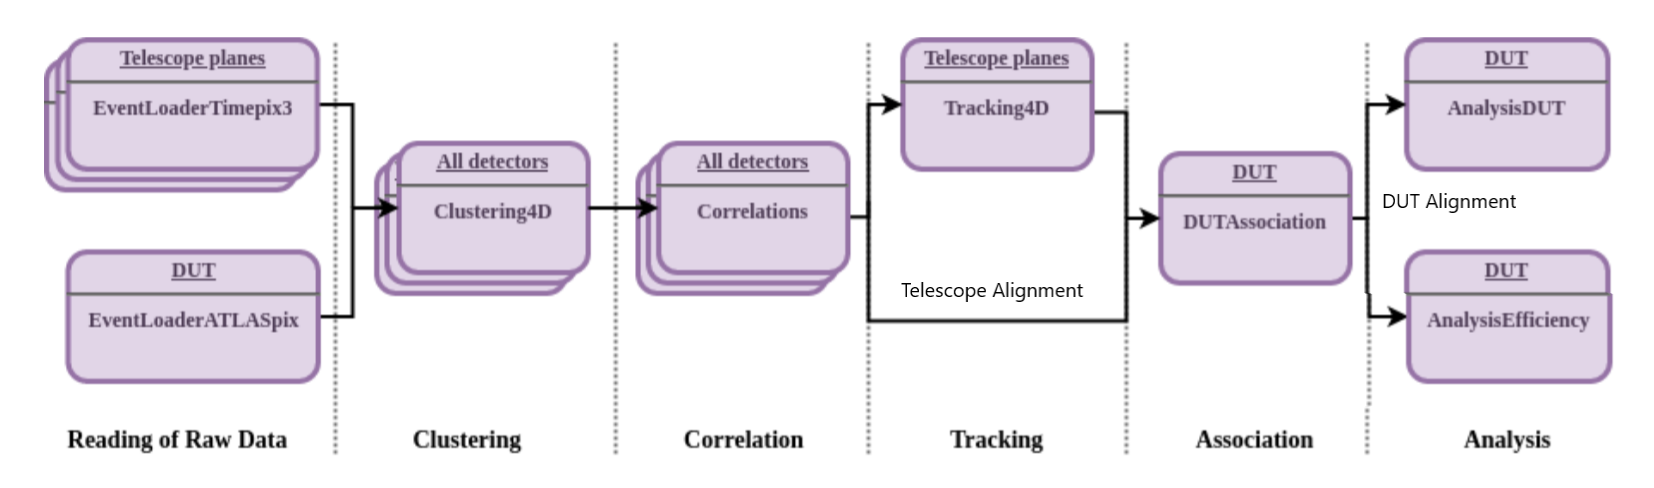
\includegraphics[height=0.3\textwidth]{images/corry.png}
  \caption{Overall track reconstruction chain with the standard clustering and tracking module. \cite{corry_track_reco}.}
  \label{fig:corry_track_reco}
\end{figure}

\chapter{Comparison of EUTelescope and Corryvreckan}\label{make}
Before using Corryvreckan to reconstruct particles for proton computed tomogrophy, it is necessary to ensure that its functioning properly
and is able to deliver equally valid results as the EUTelescope framework.
The chosen data sample is batch 3 of a DESY testbeam run from june 2020. Besides the six Mimosa26 sensors it contains two RD53a sensors
as DUT's inbetween the triplets and a FEI4 sensor as a time reference behind the telescope. The RD53a sensors are pixel sensors
manufactured in a $\SI{65}{\nano\meter}$ CMOS technology with a matrix of (400 $\times$ 192) \textmu m$^2$ pixels of
(50 $\times$ 50) \textmu m$^2$ size. Electrons with an energy of $\SI{5}{\GeV}$ were used to to irradiate the sensors.
To compare the two softwares, results of each individual
reconstruction step is analysed. \\

\section{Clustering}
After converting the hit information to their respective formats, the clustering is the first step performed by Corryvreckan and EUTelescope
to be investigated.
It should be noted that no cut on the firing frequency is applied in any of the softwares in order to properly investigate
the their similarity, as the cut on the frequency in both frameworks is not defined similarly.
In figure \ref{fig:cluster_size} the determined cluster sizes of Corryvreckan and EUTelescope are shown for the first plane exemplary.
For both softwares, the charge weighted center of gravity algorithm is used.

\begin{figure}
  %\centering
  \hspace{-2.5cm}
  \begin{subfigure}{0.62\textwidth}
      %\centering
      \includegraphics[height=0.82\textwidth]{plots/june_clustersize_tel1_corry.pdf}
  \end{subfigure}
  \begin{subfigure}{0.62\textwidth}
      %\centering
      \hspace{0.9cm}
      \includegraphics[height=0.82\textwidth]{plots/june_clustersize_tel1_EU.pdf}
  \end{subfigure}
  \caption{Number of clusters of different sizes calculated by Corryvreckan shown on the left and EUTelescope shown on the right.}
  \label{fig:cluster_size}
\end{figure}

The number of identified clusters is identical and the distribution looks similar implying an identical clustering process
and no differences due to the data conversion step. A closer look at the individual bin entries, shown in table ..., confirms that the
distributions are identical.

\chapter{Simulation studies for proton computed tomogrophy}



\section{The simulation software Allpix$^2$}
Allpix$^2$ is a generic simulation framework developed at CERN to simulate the performance of silicon detectors and was released in 2017. It builds upon the
Geant4 \cite{geant4} package to perform tasks in the simulation chain. The main tasks of Allpix$^2$ is the simulation of energy depostions of particles
in the sensors, the propagation of charge carriers in the sensor material and the digitization of the signal. It has a modular
structure to ensure an easy handling, while still allowing for complex detector simulations. Instantiation and processing of the modules is done by the core of the framework,
which contains five subsystems. This includes the configuration containing the configuration manager, which grants access to the configuration file, the
module subsystem, which loads and executes the modules and the geometry subsystem, which provides the information of the telescope setup. Objects are transferred
from one module to another with the messenger subsystem.
Figure \ref{fig:allpix} depicts the overall structure of Allpix$^2$.

\begin{figure}
  \centering
  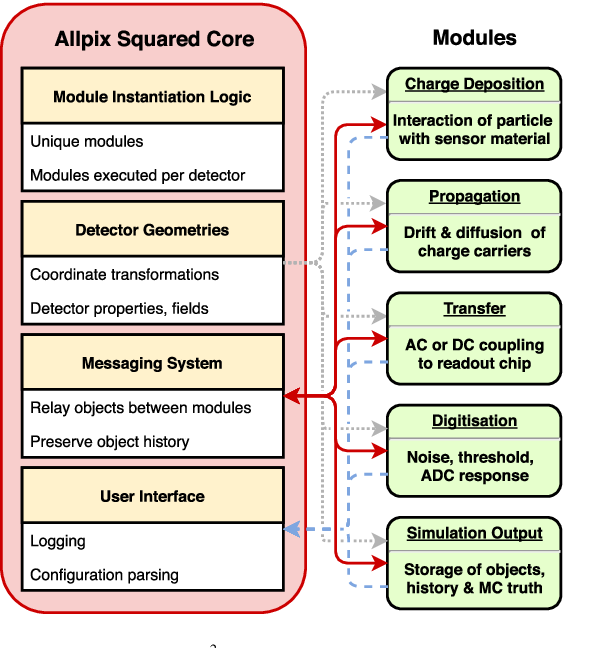
\includegraphics[height=0.5\textwidth]{images/allpix.png}
  \caption{Schematic representation of the overall Allpix$^2$ structure. \cite{fig_allpix}.}
  \label{fig:allpix}
\end{figure}

The telescope geometry has to be specified in a geometry file, which includes all sensors and their pixel matrix as well as their spatial and time resolution. Additionally,
the position and orientation have to be stated. Optionally, uncertainties on the position and orientation can be set to account for misalignment in real telescope setups.
In the configuration file, the geometry is imported as well as the modules for the simulation in order of execution, which
will be explained in the following.

The world frame of the simulation is created with the GeometryBuilderGeant4 module. The world material can be either air or vacuum with a configurable world margin percentage.
Afterwards all detectors from the internal detector models and passive material models are created according to the specifications in the geometry file.

Charge carriers are deposited in the active volume with the DepositionGeant4 module, which initializes the simulation of particles. The shape of the source beam, as well
as the type of particle and its energy can be specified. Further parameters are the width of the beam, its angular distribution based on a gaussian distribution and the energy
uncertainty of the simulated particles. All particles created at the same time define an event. The number of generated electron hole pairs is calculated with the
mean pair creation energy and is subject to fluctuations, which are defined by the fano factor.

An electric field is added to the sensors with the ElectricFieldReader module. By default all sensors are targeted by the module, though specific sensors can be stated.
There are three types of electric field models available, constant electric fields, linear electric fields and external simulated electric fields, with only
linear electric fiels being used in the scope of this thesis. The constant slope of linear electirc fields are defined by the bias voltage and the
depletion voltage of the sensor. Optionally, the depletion depth instead of the depletion voltage can be specified.

Either with the ProjectionPropagation or the GenericPropagation module the transport of charge carriers through the sensitive material are simulated.
The first module projects electrons or hole onto the surface and performs a randomized diffusion based on a two dimensional gaussian distribution around
the projection. Using an approximation of the drift time makes it possible to determine the diffusion width under the assumption of a linear electric field. This
module save computing time at the cost of accuracy. \\
The GenericPropagation module consists of a combined simulation of diffusion and drift calculated with a Runge-Kutter-Fehlberg method.
It is compatible with any electric field model and can simulate both electrons and holes
at the same time making the module
more accurate at the cost of computing time. The integration time can be specified by the user to determine the time of the propagation process. \\
In both modules, charge carriers are combined to sets and propagated together with no interaction between them. The set size of charge carriers can be specified by the user,
making it possible to control the accuracy and computing time of the simulation. For diffusion simulations it is necessary to specifiy the temperature of the sensor material
to calculate the diffusion constant.

Sets of charges are combined on the sensor pixels with the SimpleTransfer module and are prepared  to be processed by the front-end chips. The
propagated charges are mapped directly to the nearest pixel, while charge carriers that are outside the pixel grid or too far away from the implants are ignored.

Collected charges are then translated into digitised signals proportional to the input charge by the DefaultDigitizer module. Additionally, gaussian noise constributions
from the readout electronics can be simulated and a signal threshold can be defined. The output signal is given in units of the electron charge per default, but
can also be given in bits by simulating a QDC converter. Optionally, a gain factor and gain smearing can be set.

Simulated events and the produced plots of the different modules are stored in a root file. With the ROOTObjectWriter module further information like propagated charge,
deposited charge, Monte Carlo (MC) particle information and pixel hit information are stored in an additional ROOT file. Allpix$^2$ also enables the storing of
data in formats compatible with the EUTelescope and Corryvreckan software with the LCIOWriter module and the CorryvreckanWriter module respectively. Both modules possess parameters, which
determine what information of the Allpix$^2$ simulation is written into the ROOT files.

\chapter{Machine learning approach for true track tagging}
Applying cuts to track features in order to differentiate between improved the ratio of true and false reconstructed tracks, slightly. A more effective
approach in classifying a track as true or false can be achieved with a machine learning algorithm for classification. Unlike one dimensional cuts, a machine learning
algorithm can be implemented to find correlations between the input feature for a more accurate identification of true tracks. The library used for
machine learning is XGBoost, which is explained in the following section.

\section{XGBoost}
XGBoost \cite{xgboost} is a gradient boosting machine learning algorithm, which primarily uses decision trees as a predictive model for classification and regession analysis.
It is used for supervised learning problems to predict a target variable $y_i$ based on the training data $x_i$ containing multiple features. The model
of XGBoost describes the mathematical structure, which determines the prediction from its input data. A linear model is a common example, where the predictions
are linear combinations of the weighted input features:
\begin{align}
  \hat{y}_i = \sum_j \Theta_j x_{ij}
\end{align}
The coefficents $\Theta$ are indefinite parameters that need to be learned from the training data. Thus, the task of training is in determining the optimal parameters
for the target variable $y_i$ based on our input $x_i$. In order to train a model, an objective function needs to be defined, which measures how well
the model fits the training data. Those functions consist of the training loss function $L(\Theta) $ and the regularization term $\Omega (\Theta)$.
\begin{align}
  \text{obj}(\Theta) = L(\Theta) + \Omega(\Theta)
\end{align}

The training loss function is commonly defined as the mean squared error or logistic loss for logisitc regression problems:
\begin{align}
  &L(\Theta) = \sum_i (y_i - \hat{y}_i)^2 \\
  &L(\Theta) = \sum_i [y_i \ln{(1 + e^{-\hat{y}_i})} + (1 - y_i) \ln{(1 + e^{-\hat{y}_i})}]
\end{align}
The regularization term describes the complexity of a model in order to prevent overfitting.

\section{Decision tree ensemble}
The model used by the XGBoost library is the decision tree ensemble, which consists of a set of classification and regression tress (CART).
A CART assigns a prediction score to each of the leaves in which the input features are classified. The prediction of a single tree is usually not accurate,
therefore the prediction of numerous trees is summed together. This method can be written mathematically as:
\begin{align}
  &\hat{y}_i = \sum_{k=1}^K f_k(x_i)\,, \: f_k \in \mathcal{F} \\
  &\text{obj}(\Theta) = \sum_i^n l(y_i, \hat{y}_i) + \sum_{k=1}^K \Omega(f_k)
\end{align}
Where $K$ is the number of trees, $\mathcal{F}$ the set of all possible CARTs and $f$ a function in $\mathcal{F}$. A decision tree ensemble is shown exemplary in
figure \ref{fig:random_forest}.

\begin{figure}
  \centering
  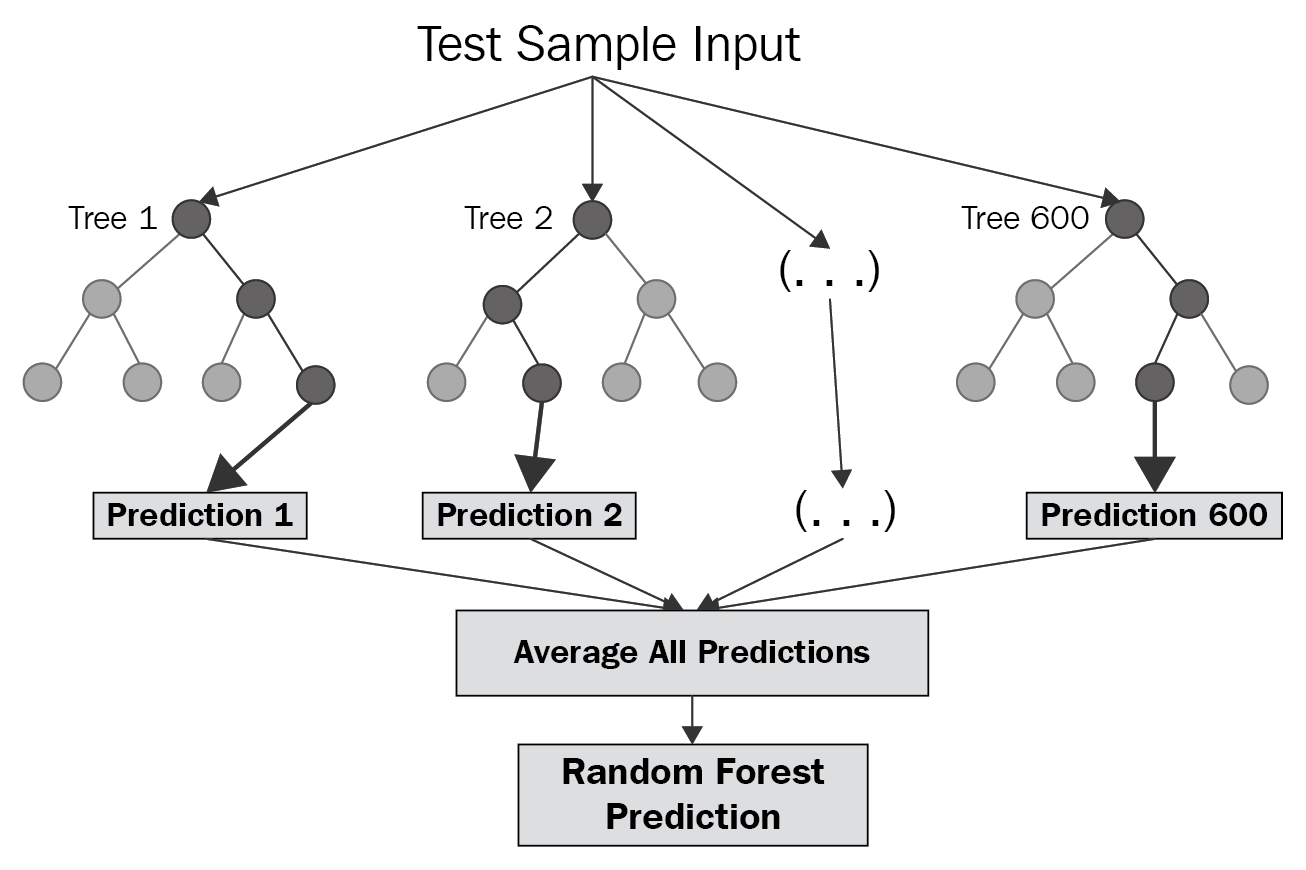
\includegraphics[height=0.6\textwidth]{images/random_forest.png}
  \caption{Representation of a decision tree ensemble \cite{random_forest}.}
  \label{fig:random_forest}
\end{figure}

\section{Boosted trees}
The model used for boosted trees and a random forest is both the tree ensembles with the only difference being the training method. Optimizing the objective functions for
boosted trees is achieved by additive training. This means that everything learned is fixed and only one new tree per step $t$ is added. This can be written
down as follows:
\begin{align}
  \hat{y}_i^{(t)} = \sum_{k=1}^t f_k(x_i) = \hat{y}_i + f_t(x_i)
\end{align}

The tree added in each step is supposed to optimize our objective. For a mean squared error loss function, the objective at step $t$ can be written as:
\begin{align}
  \text{obj}^{(t)} &= \sum_{i=1}^n \left[g_i f_t(x_i)] + \frac{1}{2}h_i f_t^2(x_i)\right] + \Omega(f_t)  \\
  g_i &= \partial_{\hat{y}_i^{(t-1)}} l(y_i, \hat{y}_i^{(t-1)}) \\
  h_i &= \partial^2_{\hat{y}_i^{(t-1)}} l(y_i, \hat{y}_i^{(t-1)})
\end{align}

The value of the objective function only depends on $g_i$ and $h_i$, giving XGBoost the advantage of using custom loss functions including logistic regression.

However, the regularization term still needs to be defined. One definition that works well in practice and thus used by XGBoost is:
\begin{align}
  \Omega (f) = \gamma T + \frac{1}{2}\lambda \sum_{j=1}^T \omega_j^2
\end{align}
Here, $\omega_{q(x)}$ is the vector of scores on leaves, $q$ is a function that assigns each data point to the corresponding leave and $T$ is the number of leaves.

With this definition, the objective function can be compressed to:
\begin{equation} \label{eqn:obj}
  \text{obj} = -\frac{1}{2}\sum_{j=1}^T \frac{G_j^2}{H_j + \lambda} + \gamma T
\end{equation}
Here, $G_j$ and $H_J4$ are the sum over all $g_i$ and $h_i$ repsectively. Equation \ref{eqn:obj} is a measure for how good a structure tree is. Its score
is determined by the statistics $g_i$ and $h_i$ in the leaves, with a smaller score meaning a better tree structure.
Since it is not feasible to enumerate all possible tress to find the best one, only one level of a tree is optimized at a time.
For each split of a leaf into a new left and right leaf, the gained score is defined as:
\begin{equation}
  \text{Gain} = \frac{1}{2}\left[\frac{G_L^2}{H_L + \lambda} + \frac{G_R^2}{H_R + \lambda} - \frac{(G_L + G_R)^2}{H_L+H_R+\lambda}\right] -\gamma
\end{equation}

Optimal splits are then determined by sorting all instances and calculate the structure score of all possible split solutions.

\section{Machine learning setup}
The data used to train the learner %is identical to the one from section \ref{sec:feature} and
consists of 400000 generated $\SI{200}{\mega\eV}$ protons with ten protons per event
traversing the telescope described in section \ref{sec:setup}. The protons
are reconstructed with Corryvreckan, with the true tracks being identified with the MC truth from Allpix$^2$ and masked for the learner. A total number of 92546 tracks
are reconstructed, with 36340 being true tracks.
To test the learner, another simulation, being identical to the one in \ref{sec:feature} is used and consists of 100000 protons with ten protons per event.

The objective of the learner is binary logistic, which performs a logistic regression and outputs a probability for classifying a track as true or false.
Therefore, a logistic loss function is used for training the model.
To determine the optimal number of boosting rounds, early stopping is utilized on a validation set, consisting of 100000 generated protons. This means, that
the model will train until the validation score stops improving for ten consecutive boosting rounds, with the number
of boosting rounds belonging to the highest validation score being chosen for testing. In this case, the validation score refers to the area under the
Receiver Operating Characteristic (ROC) curve. \\
The ROC curve describes the true positive rate $TPR = t_p/(t_p + f_p)$ as a function of the false positive rate $FPR = f_p/(f_p + t_n)$ with
$t_p$, $t_n$ and $f_p$ meaning the true positive, true negative and false positive classification of a track respectively. The larger the area under the curve (auc) in respect
to the diagonal, which represents random classification, the better the performance of the classificator. \\
All features, including $\chi^2$, kink angles, cluster positions and charge depositions are selected as input for the classifier. Less useful features
may not contribute significantly for classification, but also do not disrupt the learning process, as trees do not split as often on variables with little impact.
Thus, no problems will arise by taking all features into account, as long as the training data is sufficiently large to be able to compensate for inefficiencies.

Tuning several hyper parameters is necessary to ensure an optimal performance of the classificator. Taking many hyper parameters and values into account, comes at the
cost of a large computation time. For this reason, four parameters are chosen to be optimised. The maximum depth of each tree influences the
complexity of the model and the likeliness of overfitting. With the learning rate $\eta$, overfitting can be prevented as it represents a weighting factor for
corrections added by new trees in the model. It takes values from zero to one, with smaller values describing smaller corrections from further trees. \\
The minimum loss reduction required for an additional partition on a leaf node is referred to as $\gamma$. A similar impact has the minimum sum of instance weight $\theta$
needed in a child. Leaf nodes with a sum of weights less than the specified value will prevent further tree partition steps.
Both the $\theta$ and $\gamma$ take values from 0 to $\infty$ and are a measure for how conservative the algorithm will be, with larger values representing a more
conservative algorithm.

A grid search from the library Scikit-learn \cite{scikit} is used to determine an optimal value for each of the parameters mentioned above. The values given as input into the grid search
are shown in table \ref{tab:grid}.

  \begin{table}
    \centering
    \begin{tabular}{c c c c}
      \toprule
      tree depth & $\eta$ & $\gamma$ & $\theta$ \\
      \midrule
      3 & 0.05 & 0.5 & 1  \\
      4 & 0.1  & 1   & 25  \\
      5 & 0.3  & 2 & 50  \\
      6 & 0.7  & 5   &  \\
    \end{tabular}
    \caption{Parameter values that are used for the grid search. The tree depth refers to the maximum depth of a tree, $\eta$ refers to the learning rate,
    $\gamma$ is a threshold for the allowed minimum loss reduction in a partition step and $\theta$ is the minimum sum of instance weight needed in a child.}
    \label{tab:grid}
  \end{table}
To quantify each different combination of the hyper parameter values, a 5-fold cross validation is performed. This means that the data set is split into five equally
large sets, with the learner training on four of them and evaluating on the last one. Each of the five sets serves as the test data, which means that for each
parameter combination five runs are performed. The area under the ROC curve serves as the scoring function to measure how good the predicition on the test data set is.
A mean of the five auc values represents the score, which is compared in the grid search. Thus, the cross validation helps to compensate for variability in the simulated
data to derive an accurate estimate of the predictive power of the model. \\
The maximal AUC of $0.579(3)$ is achieved with a maximum tree depth of 5, $\eta=0.7$, $\gamma=5$ and $\theta=25$. With $\gamma=5$, the result of the grid search of the remaining
parameters can be visualized and is shown in figure \ref{fig:grid}

\begin{figure}
  \centering
  \includegraphics[height=0.6\textwidth]{plots/grid_search.pdf}
  \caption{The mean test score referring to the auc for the different hyper parameter configurations with the errorbars being the standard deviation of the mean. The
  smaller bars refer to $\eta$, the larger bars to $\theta$ and the red marked value to the maximal AUC.}
  \label{fig:grid}
\end{figure}

Varying the values of the hyper parameters only causes small changes in the mean test score, especially the learning rate has a negligible influence on the AUC. Taking the
standard deviations into account makes it impossible to determine, wether the best combination of hyper parameters actually have the highest AUC. However, due to the
small differences, no significant impact is to be expected in this case. For that reason, the above mentioned hyper parameter values are chosen for training and testing the model.

\section{Machine learning results}
To compare the performance of the learner on the train and test data, the normalised distribution of the output probabilities are investigated.
These are shown in figure \ref{fig:output} alongside the corresponding differences.

\begin{figure}
  \hspace{-2.5cm}
  %\centering
  \begin{subfigure}{0.62\textwidth}
      \centering
      \includegraphics[height=0.82\textwidth]{plots/output_normed.pdf}
  \end{subfigure}
  \begin{subfigure}{0.62\textwidth}
      %\centering
      \hspace{0.95cm}
      \includegraphics[height=0.82\textwidth]{plots/output_difference.pdf}
  \end{subfigure}
  \caption{Normalised probabilitiy distributions of tracks being true and false for the train and test data set shown on the left.
  The corresponding differences between the performance on the training and testing data is shown on the right.}
  \label{fig:output}
\end{figure}

The distribtions of the train and test data predictions show small differences, indicating that no signifiacnt overtraining occurs during the training process.
%For both true and false tracks, the greatest deviations are found at their most probable value, between 0.8 and 0.9.
Both true and false tracks have a maximum around 0.8 as their most probable value, though the peak for the true tracks is higher due to the larger number
of false tracks assigned to small probabilities of being true. Also noteworthy is, that a neglicable number of tracks have a probability of 0.9 and higher. This means that
with the given input, a lot of false combinations of clusters still show similar properties to true tracks.

\chapter{Summary and Outlook}
The performance of Corryvreckan was analysed and compared to EUTelescope in the scope of this thesis. Furthermore, the reconstruction of low energy proton
tracks with the use of Corryvreckan was investigated.\\
With the track reconstruction of beam test data, Corryvreckan proved to produce equally valid results in comparison to the EUTelescope framework. No differences
arise in their data conversion and clustering process. A different structure of the tracking and alignment process of the frameworks causes a distinction in the residuals
of the telescope plane. The residual means of the telescope planes are below $\SI{1}{\micro\meter}$ for both softwares, indicating successful telescope alignments.
With standard deviations of $4.450(4)$\,\textmu m\, for Corryvreckan and $3.972(3)$\,\textmu m\, for EUTelescope, shown for the second sensor exemplary, the
reconstrcuted spatial resolutions proved to be well within
the expected value of $\sigma_{\text{M26}} = \SI{18.4}{\micro\meter}/\sqrt{12} \approx \SI{5.311}{\micro\meter}$ for Mimosa26 sensors. The noticebly smaller values
arise due to the used centre-of-gravity algorithm for the calculation of cluster centres. \\
Similar results are also seen for the DUT residuals, shown for the FEI4 sensor in this thesis, as only a third of the RD53a sensor volume was depleted during the beam test measurement.
An alignment below $\SI{1}{\micro\meter}$ was achieved for both frameworks with standard deviatons of $21.22(4)$\,\textmu m\, and $22.17(4)$\,\textmu m\, in horizontal direction and
$72.3(2)$\,\textmu m\, and $72.7(2)$\,\textmu m\, in vertical direction for Corryvreckan and EUTelescope respectively. With expected spatial resolutions of
$\sigma_{\text{FEI4},\text{x}} \approx \SI{14.434}{\micro\meter}$ and $\sigma_{\text{FEI4},\text{y}} \approx \SI{72.169}{\micro\meter}$ for cluster centres calculated by
arithmetic mean, both frameworks determined a similar, but non optimal value for the horizontal residual of the sensor. (...) \\
Thus, the results of the reconstruction chain upto the
association of clusters from the DUT planes are similar for the two softwares. Due to the minimization of external dependencies and the more user friendly structure of
Corryvreckan in comparison to EUTelescope, the former is suitable to supersede the EUTelescope framework for track reconstruction in beam test experiments. \\
Some uses of Corryvreckan, especially alternative modules, were not in the focus of this thesis,
as they were not necessary for further analysis of proton track reconstruction. This includes the determination of the
efficiency of sensors with the AnalysisEfficiency module. Since EUTelescope is not designed to calculate sensor efficiencies, the TBMon2 software was used in the past in addition
to EUTelescope. This opens up the possibility for Corryvreckan to also replace the TBMon2 software, making the track reconstruction and analysis process more efficient.

The reconstruction of simulated protons of different energy with Corryvreckan produced the expected results. Due to no misalignments of sensors in the telescope and uncertainties
in the protons energy, the residuals for high energy protons form sharp peaks. Since, the used IBL sensors have a different spatial resolution, a five-peak structure
forms, which starts to blur into one residual peaks for lower energies below $\SI{1}{\giga\eV}$, due to stronger scattering of the protons. For even lower energies,
around $\SI{200}{\mega\eV}$, the number of reconstructed tracks decrease significantly, as fewer protons deposit energy in all six planes. Since these energies are
used for proton therapy, and a sufficient number of reconstructed protons are necessary to cretae a proton computed tomography image, the patient
will need to be irradiated for longer times to compensate for the small number of reconstructed tracks. However, only small amount of energy is deposited by protons, while traversing
the human body, making longer radiation steps for pct possible without significantly damaging healthy tissue. \\
A greater problematic arises from the high track density of the proton beams causing large track mutiplicities and thus a large number of tracks with false combinations of
clusters. Falsely reconstructed tracks will lower the resolution of the pct image and therefore have to be reduced to a minimum. Using stronger spatial cuts and higher
opening angles for the proton beam increased the ratio of true and false tracks by (...) respectively, while the number of true tracks decreases significantly. Due to the loss of
true tracks for increasingly stricter spatial cuts and larger opening angles, the use of these parameters to improve the ratio is limited for the use of pct. \\
Cuts on track features proved to be useful for the $\chi^2$ value and the horizontal kink angles of the third and fourth plane. The optimal combination of cuts, determined
with a grid search, result in a ratio of 0.477. (...)

With the utilisation of a boosted decision tree used for the classification of tracks, the true and false positive rates achieved with the machine learner are better
than any of the previous methods, including the grid search. The resulting AUC of the test data set is 0.756, with the same data set having AUC's of
0.615, 0.617 and 0.587 for the cut on the $\chi^2$, $\phi_{x,3}$ and $\phi_{x,4}$ respectively. (...)
However, a significant amount of false tracks are still classified to be true
with a high probability, which means that the input features do not enable an optimal classification. Thus, the most crucial step to optimise the classification of the machine learner is
to determine further input features. \\

Another option is to improve the reconstruction process of Corryvreckan with more advanced track finding algorithms. The Tracking4D module uses a straight line as the initial track for
the track finding process. The newer TrackingMultiplet module fits two straight lines, one through each triplet, and connects them at a specified position with an arbitrary kink.
A full track forms by connecting the upstream and downstream tracks with the lowest distance and within specifed cuts, allowing for further rejection of false combinations
of clusters.


%\appendix
% Hier beginnt der Anhang, nummeriert in lateinischen Buchstaben
\chapter{Appendix}
%\section{Bin entries of cluster size plots}
  \begin{table}
    \centering
    \begin{tabular}{c | c c}
      \toprule
      Bin & Corryvreckan & EUTelescope \\
      \midrule
      1      & 3934209 & 3934209            \\
      2      & 1136782 & 1136782           \\
      3      & 295505  & 295505           \\
      4      & 288595  & 288595           \\
      5      & 50477   & 50477           \\
      6      & 42916   & 42916           \\
      7      & 31800   & 31800           \\
      8      & 23759   & 23759           \\
      9      & 15892   & 15892           \\
      10     & 11378   & 11378           \\
      11     & 8030    & 8030           \\
      12     & 7472    & 7472           \\
      13     & 5576    & 5576           \\
      14     & 4332    & 4332           \\
      15     & 3155    & 3155           \\
      16     & 3740    & 3740           \\
      17     & 2744    & 2744           \\
      18     & 1917    & 1917           \\
      19     & 1357    & 1357           \\
      20     & 1022    & 1022           \\
      21-30  & 990434  & 990434            \\
      31-40  & 634     & 634       \\
      41-50  & 986247  & 986247        \\
      51-59  & 207     & 207            \\
    \end{tabular}
    \caption{Bin entries of the cluster size plots of Corryvreckan and EUTelescope for the first plane shown in figure \ref{fig:cluster_size}.}
    \label{tab:cluster_sizes}
  \end{table}

\clearpage

\begin{lstlisting}[caption={Configuration file of Corryvreckan for the testbeam anaylsis of June 2020 Batch 3}]
[Corryvreckan]
detectors_file = output/updated_real_geometry.conf
detectors_file_updated = output/updated_real_geometry.conf
histogram_file=histogram_testbeam_realdata.root

[EventLoaderEUDAQ]
file_name = "/path_to_data.raw"
long_detector_id = false

[Clustering4D]

[Correlations]

[Prealignment]
method= gauss_fit

[Tracking4D]
track_model = "gbl"
exclude_dut = true
spatial_cut_abs = 120um, 120um
timing_cut_abs = 350ns
min_hits_on_track = 6
momentum = 5GeV

[AlignmentTrackChi2]
iterations = 3

[DUTAssociation]
spatial_cut_abs =500um, 200um
time_cut_abs = 230us

[AlignmentDUTResidual]
iterations = 3

[AnalysisDUT]
chi2ndof_cut = 5
\end{lstlisting}

\clearpage
\begin{lstlisting}[caption={Detector file of Corryvreckan for the testbeam anaylsis of June 2020 Batch 3}]
[plane0]
material_budget = 0.00075
number_of_pixels = 1152, 576
orientation = -0.659875deg,5.4639deg,0.350077deg
orientation_mode = "xyz"
pixel_pitch = 18.4um,18.4um
position = -658.122um,-147.97um,0
spatial_resolution = 5.4um,5.4um
time_resolution = 230us
type = "mimosa26"

[plane1]
material_budget = 0.00075
number_of_pixels = 1152, 576
orientation = -0.47332deg,4.61982deg,-0.117972deg
orientation_mode = "xyz"
pixel_pitch = 18.4um,18.4um
position = -587.717um,-133.671um,111mm
spatial_resolution = 5.4um,5.4um
time_resolution = 230us
type = "mimosa26"

[plane2]
material_budget = 0.00075
number_of_pixels = 1152, 576
orientation = -0.136822deg,3.69758deg,0.117857deg
orientation_mode = "xyz"
pixel_pitch = 18.4um,18.4um
position = -386.259um,-237.934um,222mm
spatial_resolution = 5.4um,5.4um
time_resolution = 230us
type = "mimosa26"

[plane110]
material_budget = 0.003
number_of_pixels = 401, 193
orientation = 8.55701deg,46.4751deg,3.61319deg
orientation_mode = "xyz"
pixel_pitch = 50um,50um
position = -6.65508mm,-83.16um,355mm
roi = [[266,1],[266,193],[401,1],[401,193]]
role = "dut"
spatial_resolution = 14um,14um
time_resolution = 200ns
type = "rd53a"

[plane112]
material_budget = 0.003
number_of_pixels = 401, 193
orientation = 0,-0,-0.0220589deg
orientation_mode = "xyz"
pixel_pitch = 50um,50um
position = -5.5818mm,448.868um,425mm
roi = [[266,1],[266,193],[401,1],[401,193]]
role = "dut"
spatial_resolution = 14um,14um
time_resolution = 200ns
type = "rd53a"

[plane3]
material_budget = 0.00075
number_of_pixels = 1152, 576
orientation = 0,0,0
orientation_mode = "xyz"
pixel_pitch = 18.4um,18.4um
position = 0,0,571mm
role = "reference"
spatial_resolution = 5.4um,5.4um
time_resolution = 230us
type = "mimosa26"

[plane4]
material_budget = 0.00075
number_of_pixels = 1152, 576
orientation = 1.15485deg,-0.940166deg,0.246945deg
orientation_mode = "xyz"
pixel_pitch = 18.4um,18.4um
position = -274.402um,134.999um,681mm
spatial_resolution = 5.4um,5.4um
time_resolution = 230us
type = "mimosa26"

[plane5]
material_budget = 0.00075
number_of_pixels = 1152, 576
orientation = 0.735678deg,-1.16597deg,-0.0280176deg
orientation_mode = "xyz"
pixel_pitch = 18.4um,18.4um
position = -482.401um,213.683um,793mm
spatial_resolution = 5.4um,5.4um
time_resolution = 230us
type = "mimosa26"

[plane21]
material_budget = 0.003
number_of_pixels = 80, 336
orientation = 179.875deg,3.70623deg,89.9804deg
orientation_mode = "xyz"
pixel_pitch = 250um,50um
position = -1.42585mm,504.062um,835mm
role = "dut"
spatial_resolution = 72um,14um
time_resolution = 25ns
type = "fei4"
\end{lstlisting}

\clearpage

\begin{lstlisting}[caption={Configuration file of EUTelescope for the testbeam anaylsis of June 2020 Batch 3}]
[DEFAULT]
# The path to this config file
BasePath                = /path_to_config_file

# Set the folder which contains the raw/native data files
NativePath              = /path_to_data_file

#The location of the steering templates
TemplatePath    = %(BasePath)s/steering-templates

# The GEAR file describing the detector geometry,
# this is passed from the runlist.csv
GearFile                = @GearGeoFile@

# Beam Energy is retrieved from the runlist.csv
BeamEnergy              = @BeamEnergy@

# Path to the GEAR files
GearFilePath    = %(BasePath)s/gear

# The XML file with histogram information
HistoInfoFile   = %(TemplatePath)s/histoinfo.xml

# Formats the output;
# @RunNumber@ is the current run number
# padded with leading zeros to 6 digits
FilePrefix              = run@RunNumber@

# Skip events in a run; set to 0 for all data
SkipNEvents             = 0

# Output subfolder structure
OutPath         = %(BasePath)s/output
DatabasePath    = %(OutPath)s/database
HistogramPath   = %(OutPath)s/histograms
LcioPath        = %(OutPath)s/lcio
LogPath         = %(OutPath)s/logs
TBTrackFilePath = %(OutPath)s/tbtrack

# Limit processing of a run to a certain number of events
MaxRecordNumber = 1000000000

# The verbosity used by the EUTelescope producers
Verbosity               = MESSAGE5

# After how many events you want a "Processing event XXXX" message
NEventsMessage  = 2500

[converter]
# How many events for noisy pixel analysis
NoOfEvents              = 100000

M26SensorVec            = 0 1 2 3 4 5
FiringFreqCutM26        = 0.005

APIXSensorVec           = 110 112 21
FiringFreqCutAPIX       = 0.001

[clustering]

[hitmaker]
# ID of fixed Sensor for correlation and alignemnt
FixedPlane              = 3

#Number of events used for Correlator and PreAligner
NoEvents                = 100000

#Residual cuts for Correlator and PreAligner
ResidualsXMin   = -3. -3. -3.  -10. -10.  -3. -3. -3.  -10.
ResidualsXMax   =  3.  3.  3.   10.  10.   3.  3.  3.   10.
ResidualsYMin   = -3. -3. -3.  -10. -10.  -3. -3. -3.  -10.
ResidualsYMax   =  3.  3.  3.   10.  10.   3.  3.  3.   10.


[alignGBL]
#Template for steering file is the same in all the alignment iterations
TemplateFile    = alignGBL-tmp.xml

MaxTrackCandidatesTotal = 100000

GearFile                = @GearGeoFile@@RunNumber@_pre.xml
Iteration               = 0

# Number of alignment constants used.
AlignMode               = XYZShiftsRotXYZ

UpstreamTriplet         = 0 1 2
LastUpstreamSensor      = 2
DownstreamTriplet       = 3 4 5

FixedPlanes             = 0 5
FixedZShift             = 0 1 2 110 112 3 4 5 21

# res = pitch/sqrt(12)
resMim                  = 0.0052
resRD531X               = 0.0289
resRD531Y               = 0.0072
resRD532XY              = 0.0144
resFEI4X                = 0.0722
resFEI4Y                = 0.0144

# Both DUTs are 50x50
ResolutionX = %(resMim)s %(resMim)s %(resMim)s %(resRD532XY)s
%(resRD532XY)s %(resMim)s %(resMim)s %(resMim)s %(resFEI4X)s
ResolutionY = %(resMim)s %(resMim)s %(resMim)s %(resRD532XY)s
%(resRD532XY)s %(resMim)s %(resMim)s %(resMim)s %(resFEI4Y)s

UpstreamTripletCut              = 0.2
DownstreamTripletCut            = 0.2
UpstreamSlopeCut                = 3.0
DownstreamSlopeCut              = 3.0
TripletMatchingCut              = 0.5
DUTCuts                         = 1.0 1.0

[alignGBL1]
#Template for steering file is the same in all the alignment iterations
TemplateFile    = alignGBL-tmp.xml

MaxTrackCandidatesTotal = 100000

GearFile  = @GearGeoFile@@RunNumber@_pre_alignGBL0.xml
Iteration = 1

#Number of alignment constants used.
AlignMode               = XYZShiftsRotXYZ

UpstreamTriplet         = 0 1 2
LastUpstreamSensor      = 2
DownstreamTriplet       = 3 4 5

FixedPlanes             = 0 5
FixedZShift             = 0 1 2 110 112 3 4 5 21

# res = pitch/sqrt(12)
resMim                  = 0.0052
resRD531X               = 0.0289
resRD531Y               = 0.0072
resRD532XY              = 0.0144
resFEI4X                = 0.0722
resFEI4Y                = 0.0144

# Both DUTs are 50x50
ResolutionX = %(resMim)s %(resMim)s %(resMim)s %(resRD532XY)s
%(resRD532XY)s %(resMim)s %(resMim)s %(resMim)s %(resFEI4X)s
ResolutionY = %(resMim)s %(resMim)s %(resMim)s %(resRD532XY)s
%(resRD532XY)s %(resMim)s %(resMim)s %(resMim)s %(resFEI4Y)s

UpstreamTripletCut              = 0.2
DownstreamTripletCut            = 0.2
UpstreamSlopeCut                = 3.0
DownstreamSlopeCut              = 3.0
TripletMatchingCut              = 0.5
DUTCuts                         = 1.0 1.0

[alignGBL2]
#Template for steering file is the same in all the alignment iterations
TemplateFile    = alignGBL-tmp.xml

MaxTrackCandidatesTotal = 100000

GearFile = @GearGeoFile@@RunNumber@_pre_alignGBL0_alignGBL1.xml
Iteration = 2

#Number of alignment constants used.
AlignMode               = XYZShiftsRotXYZ

UpstreamTriplet         = 0 1 2
LastUpstreamSensor      = 2
DownstreamTriplet       = 3 4 5

FixedPlanes             = 0 5
FixedZShift             = 0 1 2 110 112 3 4 5 21

# res = pitch/sqrt(12)
resMim                  = 0.0052
resRD531X               = 0.0289
resRD531Y               = 0.0072
resRD532XY              = 0.0144
resFEI4X                = 0.0722
resFEI4Y                = 0.0144

# Both DUTs are 50x50
ResolutionX  = %(resMim)s %(resMim)s %(resMim)s %(resRD532XY)s
%(resRD532XY)s %(resMim)s %(resMim)s %(resMim)s %(resFEI4X)s
ResolutionY  = %(resMim)s %(resMim)s %(resMim)s %(resRD532XY)s
%(resRD532XY)s %(resMim)s %(resMim)s %(resMim)s %(resFEI4Y)s

UpstreamTripletCut              = 0.03
DownstreamTripletCut            = 0.03
UpstreamSlopeCut                = 2.00
DownstreamSlopeCut              = 2.00
TripletMatchingCut              = 0.20
DUTCuts                         = 0.3 0.3

[fitGBL]
#Template for steering file is the same in all the alignment iterations
TemplateFile    = fitGBL-tmp.xml

GearFile = @GearGeoFile@@RunNumber@_pre_alignGBL0_alignGBL1_alignGBL2.xml

UpstreamTriplet         = 0 1 2
LastUpstreamSensor      = 2
DownstreamTriplet       = 3 4 5

#Planes which should be excluded from track fitting:
DUTPlanes               = 110 112 21

# res = pitch/sqrt(12)
resMim                  = 0.0052
resRD531X               = 0.0289
resRD531Y               = 0.0072
resRD532XY              = 0.0144
resFEI4X                = 0.0722
resFEI4Y                = 0.0144

# Both DUTs are 50x50
ResolutionX = %(resMim)s %(resMim)s %(resMim)s %(resRD532XY)s
%(resRD532XY)s %(resMim)s %(resMim)s %(resMim)s %(resFEI4X)s
ResolutionY = %(resMim)s %(resMim)s %(resMim)s %(resRD532XY)s
%(resRD532XY)s %(resMim)s %(resMim)s %(resMim)s %(resFEI4Y)s

UpstreamTripletCut              = 0.03
DownstreamTripletCut            = 0.03
UpstreamSlopeCut                = 2.00
DownstreamSlopeCut              = 2.00
TripletMatchingCut              = 0.20
DUTCuts                         = 0.3 0.3

OutputPlanes    = 110 112 21
\end{lstlisting}

\begin{lstlisting}[caption={Allpix$^2$ simulation for 50000 protons with an energy of $\SI{100}{\giga\eV}$}]
[Allpix]
log_level = "WARNING"
log_format = "DEFAULT"
detectors_file = path_to_detector_file.conf
number_of_events = 50000
random_seed_core = 0
random_seed = 0

[GeometryBuilderGeant4]
world_material = "air"
world_margin_percentage = 0

[DepositionGeant4]
physics_list = QBBC
particle_type = "proton"
source_energy = 100GeV
source_position = 0 0 -200cm
source_type = "beam"
beam_divergence = 0mrad 0mrad
beam_size = 3mm
beam_direction = 0 0 1
number_of_particles = 1
max_step_length = 1um

[ElectricFieldReader]
type= "ibl_planar"
model="linear"
bias_voltage= -100V
depletion_depth= 200um

[GenericPropagation]
type = "ibl_planar"
temperature = 293K
charge_per_step = 300

[SimpleTransfer]
type = "ibl_planar"
max_depth_distance = 250um

[DefaultDigitizer]
type = "ibl_planar"
\end{lstlisting}

\begin{lstlisting}[caption={Allpix$^2$ geometry file for all simulations}]
[telescope0]
type = "ibl_planar"
position = 0 0 -44cm
orientation = 0deg 0 0

[telescope1]
type = "ibl_planar"
position = 0 0 -37cm
orientation = 0deg 0deg 90deg

[telescope2]
type = "ibl_planar"
position = 0 0 -30cm
orientation = 0deg 0 0

[dut0]
type = "ibl_planar"
position = 0 0 10cm
orientation = 0deg 0 0

[telescope3]
type = "ibl_planar"
position = 0 0 50cm
orientation = 0deg 0 0

[telescope4]
type = "ibl_planar"
position = 0 0 57cm
orientation = 0deg 0deg 90deg

[telescope5]
type = "ibl_planar"
position = 0 0 64cm
orientation = 0deg 0 0
\end{lstlisting}


\backmatter
\printbibliography

%\cleardoublepage
%\thispagestyle{empty}
\section*{Danksagung}

An dieser Stelle möchte ich mich bei all denjenigen bedanken, die mich während
der Anfertigung meiner Masterarbeit unterstützt haben. \\
Zunächst möchte ich mich bei Dr. Jens Weingarten bedanken, der die Erstkorrektur dieser Arbeit übernommen hat und mir stets wichtige Denkanstöße
gegeben hat.\\
Weiter möchte ich mich bei Dr. Kevin Kröninger bedanken, dass er mir ermöglichte an diesem Lehrstuhl meine Masterarbeit zu schreiben. \\
Ebenso gilt mein Dank den Mitgliedern der Detektor Upgrade Abteilung die mich schon zu meinen Bachelorzeiten herzlich in ihren Reihen willkommen hieß. \\
Auch den restlichen Mitgliedern des Lehrstuhls danke ich herzlich für den regen und konstruktiven Austausch in unseren wöchentlichen Meetings.

Dr. Johannes Albrecht danke ich für die Übernahme der Zweitkorrektur.

Ein besonderer Dank gilt meiner Betreuerin Valerie, welche mich mit beeindruckendem Engagement in diesem Jahr begleitet hat. Ohne ihre Unterstützung wäre
diese Arbeit und auch mein erster Testbeam am DESY nicht möglich gewesen.

Auch möchte ich mich bei Florian, Jan Lukas, Olaf und den übrigen Teilnehmer des ML Meetings für ihre Expertise danken, mit der ich meine Arbeit zu einem vernünftigen
Abschluss bringen konnte. \\
Für die verlässliche Hilfe mit der Corryvreckan Software bedanke ich mich bei Sejla Hadzic, Simon Spannagel, Jens Kröger und Paul Schütze, dessen Tür immer
offen für meine Fragen waren.

Zuletzt möchte ich mich bei meiner Familie und meinen Freunden für den motivierenden Beistand
während meines gesamten Studiums bedanken.

%\cleardoublepage
%\thispagestyle{empty}
\section*{Eidesstattliche Versicherung}
Ich versichere hiermit an Eides statt, dass ich die vorliegende Abschlussarbeit mit dem Titel \enquote{\thetitle} selbstständig und ohne unzulässige fremde Hilfe erbracht habe.
Ich habe keine anderen als die angegebenen Quellen und Hilfsmittel benutzt, sowie wörtliche und sinngemäße Zitate kenntlich gemacht. 
Die Arbeit hat in gleicher oder ähnlicher Form noch keiner Prüfungsbehörde vorgelegen.

\vspace*{1cm}\noindent
\begin{center}
  \begin{tabular}{@{}p{0.4\textwidth}@{\hspace{0.15\textwidth}}p{0.4\textwidth}@{}}
  \rule{\linewidth}{0.25pt}& \rule{\linewidth}{0.25pt}\\
  Ort, Datum & Unterschrift
  \end{tabular}
\end{center}

\subsection*{Belehrung}
Wer vorsätzlich gegen eine die Täuschung über Prüfungsleistungen betreffende Regelung einer Hochschulprüfungsordnung verstößt, handelt ordnungswidrig.
Die Ordnungswidrigkeit kann mit einer Geldbuße von bis zu \SI[round-mode=places, round-precision=2]{50000}{€} geahndet werden. 
Zuständige Verwaltungsbehörde für die Verfolgung und Ahndung von Ordnungswidrigkeiten ist der Kanzler/die Kanzlerin der Technischen Universität Dortmund. 
Im Falle eines mehrfachen oder sonstigen schwerwiegenden Täuschungsversuches kann der Prüfling zudem exmatrikuliert werden \mbox{(\S\,63 Abs. 5 Hochschulgesetz --HG--).}

Die Abgabe einer falschen Versicherung an Eides statt wird mit Freiheitsstrafe bis zu 3 Jahren oder mit Geldstrafe bestraft.

Die Technische Universität Dortmund wird ggf.\ elektronische Vergleichswerkzeuge (wie z.\,B.\ die Software \enquote{turnitin}) zur Überprüfung von Ordnungswidrigkeiten in Prüfungsverfahren nutzen. \\[\baselineskip]

\noindent Die oben stehende Belehrung habe ich zur Kenntnis genommen.\\[1cm]
\begin{center}
\begin{tabular}{@{}p{0.4\textwidth}@{\hspace{0.15\textwidth}}p{0.4\textwidth}@{}}
\rule{\linewidth}{0.25pt}& \rule{\linewidth}{0.25pt}\\
Ort, Datum & Unterschrift
\end{tabular}
\end{center}

\end{document}
